\documentclass[a4paper]{article}
\usepackage{import}
\usepackage{graphicx}
\usepackage{float}
\usepackage{pgfplots}
\usepackage{listings}
\usepackage{enumitem}
\usepackage{tikz}
\usetikzlibrary{decorations.pathreplacing} % for angle arc
\usetikzlibrary{angles, quotes, calc, positioning, trees} % for drawing angles
\pgfplotsset{compat=1.18,width=10cm}
\usepackage{tikz-cd}
\usepackage{booktabs}
\usepackage{cancel}
\usepackage{amsmath}
\usepackage{csquotes}
\usepackage{gensymb}
\usepackage{forest}
\usepackage{amsthm}
\usepackage{amssymb}
\usepackage{pgfplots}
\usepackage{lipsum}
\usepackage{mdframed} 
\usepackage{color}   
\usepackage{hyperref}
\newmdtheoremenv{theo}{Theorem}
\usepackage{mathtools}
\DeclarePairedDelimiter\ceil{\lceil}{\rceil}
\DeclarePairedDelimiter\floor{\lfloor}{\rfloor}

\hypersetup{
    colorlinks=true, %set true if you want colored links
    linktoc=all,     %set to all if you want both sections and subsections linked
    linkcolor=black,  %choose some color if you want links to stand out
}

% Define theorem styles
\newtheorem{theorem}{Theorem}[section]    % Theorems numbered within sections
\newtheorem{lemma}[theorem]{Lemma}        % Lemmas use the same counter as theorems
\newtheorem{corollary}[theorem]{Corollary} % Corollaries use the same counter as theorems
\newtheorem{proposition}[theorem]{Proposition} % Proposition uses the same counter
\newtheorem{property}[theorem]{Property}
\theoremstyle{definition}
\newtheorem{definition}[theorem]{Definition} % Now uses the same counter as theorems


% Remark-style theorem
\theoremstyle{remark}
\newtheorem{remark}[theorem]{Remark}

% Boxed environment for theorems
\newmdenv[
  linewidth=0.8pt,
  roundcorner=5pt,
  linecolor=black,
  backgroundcolor=white!5,
  skipabove=\baselineskip,
  skipbelow=\baselineskip,
  innerleftmargin=10pt,
  innerrightmargin=10pt,
  innertopmargin=5pt,
  innerbottommargin=5pt
]{thmbox}

% Custom proof environment (also boxed)
\renewenvironment{proof}[1][Proof]{%
  \begin{mdframed}[linewidth=0.8pt, roundcorner=5pt, linecolor=black, skipabove=\baselineskip, skipbelow=\baselineskip, innertopmargin=5pt, innerbottommargin=5pt]%
  \noindent\textbf{#1. }%
}{%
  \end{mdframed}%
}

% Redefine theorem environments to use thmbox
\let\oldtheorem\theorem
\renewenvironment{theorem}{\begin{thmbox}\begin{oldtheorem}}{\end{oldtheorem}\end{thmbox}}

\let\oldlemma\lemma
\renewenvironment{lemma}{\begin{thmbox}\begin{oldlemma}}{\end{oldlemma}\end{thmbox}}

\let\oldcorollary\corollary
\renewenvironment{corollary}{\begin{thmbox}\begin{oldcorollary}}{\end{oldcorollary}\end{thmbox}}

\let\oldproposition\proposition
\renewenvironment{proposition}{\begin{thmbox}\begin{oldproposition}}{\end{oldproposition}\end{thmbox}}

\let\oldproperty\property
  \renewenvironment{property}{\begin{oldproperty}}{\end{oldproperty}}


% Reference shortcuts
\newcommand{\thmref}[1]{Theorem~\ref{#1}}
\newcommand{\lemref}[1]{Lemma~\ref{#1}}
\newcommand{\corref}[1]{Corollary~\ref{#1}}
\newcommand{\propref}[1]{Property~\ref{#1}} 

% To customize QED symbol
\renewcommand{\qedsymbol}{$\blacksquare$}

\usetikzlibrary{decorations.pathreplacing} % for angle arc
\usetikzlibrary{angles, quotes, calc} % for drawing angles

\usepackage{color}   %May be necessary if you want to color links
\usepackage{hyperref}
\hypersetup{
    colorlinks=true, %set true if you want colored links
    linktoc=all,     %set to all if you want both sections and subsections linked
    linkcolor=black,  %choose some color if you want links to stand out
}

\usepackage{xcolor}
\usepackage[most]{tcolorbox}
% Define a custom tcolorbox environment for examples
\newtcolorbox{examplebox}[2][]{
  colback=blue!5!white,
  colframe=blue!30!black,
  title=#2,
  boxrule=0mm,
  fonttitle=\bfseries,
  width=\textwidth,
  breakable,
  #1
}

\newtcolorbox{definizione}[2] {
  colback=green!5!white,
  colframe=green!30!black,
  title=#2,
  boxrule=0mm,
  fonttitle=\bfseries,
  width=\textwidth,
  breakable,
  #1
}

\definecolor{codegreen}{rgb}{0,0.6,0}
\definecolor{codegray}{rgb}{0.5,0.5,0.5}
\definecolor{codepurple}{rgb}{0.58,0,0.82}
\definecolor{backcolour}{rgb}{0.95,0.95,0.92}

\lstdefinestyle{mystyle}{
    backgroundcolor=\color{backcolour},   
    commentstyle=\color{codegreen},
    keywordstyle=\color{magenta},
    numberstyle=\tiny\color{codegray},
    stringstyle=\color{codepurple},
    basicstyle=\ttfamily\footnotesize,
    breakatwhitespace=false,         
    breaklines=true,                 
    captionpos=b,                    
    keepspaces=true,                 
    numbers=left,                    
    numbersep=5pt,                  
    showspaces=false,                
    showstringspaces=false,
    showtabs=false,                  
    tabsize=2
}

\lstset{style=mystyle}

\makeatletter
\renewcommand*\env@matrix[1][*\c@MaxMatrixCols c]{%
  \hskip -\arraycolsep
  \let\@ifnextchar\new@ifnextchar
  \array{#1}}
\makeatother


\onehalfspacing
\title{Fondamenti di Informatica}
\author{Università di Verona\\Imbriani Paolo - VR500437\\Professor Isabella Mastroeni}

\begin{document}

\begin{figure}
    \centering
    \includegraphics[width=0.3\textwidth]{../UniversityofVerona.png}
    \label{fig:centered-image}
\end{figure}

\maketitle

\pagebreak

\tableofcontents

\pagebreak

\section{Cosa è l'informatica?}

La domanda chiave di questo corso è: \textit{``Cosa è l'informatica?''}. 
Ci sono diversi definizioni a seconda del contesto, ma in generale l'informatica è lo studio dei processi che trasformano l'informazione.
Possiamo vedere, storicamente, diverse definizioni come quella in inglese come "Computer Science" che vede
l'informatica come studio della calcolabilità, della computazione e dell'informazione.

\subsection{Perché la calcolabilità}

Si studia la calcolabilità perché ci aiuta a capire cosa possiamo fare con gli strumenti che abbiamo.
Quando descriviamo un programma, quanto tempo ci mette e quanto spazio utilizza è una domanda importante 
per capire se il programma è efficiente o meno. Anche in senso dei linguaggi di programmazione per capire se usiamo
quello giusto per il problema che stiamo cercando di risolvere. Chiaramente è un qualcosa che in continuo
sviluppo perché si evolve in base alla tecnologia che abbiamo a disposizione.
\\
\\
Uno dei pionieri è stato \textbf{Hilbert} che si chiedeva se la matematica fosse formalizzabile come insieme
finito (non contraddittorio) di assiomi? Godel dimostrò che non è possibile rappresentare la matematica 
come un insieme finito di assiomi in maniera non contradditoria, dicendo che in ogni sistema formale
ci sono proposizioni vere che non possono essere dimostrate all'interno del sistema.
\\
\\
Nel tentativo di rispondere a queste (ed altre) domande si è costruito un modello che 
permette di comprendere profondamente ilr agionamento computazionale,
permettendo di applicarlo ad ogni disciplina.
Cosa è calcolabile e cosa non lo è? 

\subsubsection{Macchina di Turing} 

Anche Turing si pose questa domanda e propose la \textbf{Macchina di Turing} come modello di calcolo.
Una sola macchina (programmabile) per tutti i problemi.
La macchina è universale (interprete):
\[Init(P,x)\ = \begin{cases}
    P(x) & \text{se } P \text{ è un programma che termina}\\
    \uparrow & \text{se } P \text{ è un programma che non termina}
\end{cases}\]
Se un problema è intuitivamente calcolabile, allora esisterà una macchina di Turing (o un dispostivo
equivalente, come il computer) in grado di risolverlo, cioè calcolarlo.
I modelli equivalenti possono essere:
\begin{itemize}
    \item Lambda calcolo 
    \item Funzioni ricorsive
    \item Linguaggi di programmazione (Turing completi)
\end{itemize}
I problemi non calcolabili sono infinitamente più numerosi di quelli calcolabili.
\subsubsection{Limiti dell'informatica}

L'informatica ha più limiti di quanto si possa pensare, definiti dall'equivalenza di Turing
e l'incompletezza di Godel che ci dicono che non possiamo risolvere tutti i problemi.
Ci sono anche limiti fisici e tecnologici come:
\begin{itemize}
    \item Dati non osservabili (teorema di Shannon)
    \item Dati non controllabili (velocità della luce)
\end{itemize}

\subsection{Basi di logica}

Alcune nozioni di logica che ci serviranno in seguito:

\begin{itemize}
    \item \textbf{Linguaggio del primo ordine:} 
    \begin{itemize}
        \item Simboli relazionali $(p,q, ...)$
        \item Simboli di funzione $(f,g, ...)$
        \item Simboli di costante $(c,d, ...)$
    \end{itemize}
    \item \textbf{Simboli logici:}
    \begin{itemize}
        \item Parentesi (,) e virgola
        \item Insieme numerabile di variabili $(v,x,...)$
        \item Connettivi logici ($\neg, \land, \lor, \rightarrow, \leftrightarrow$)
        \item Quantificatori ($\forall, \exists$)
    \end{itemize}
    \item \textbf{Termini:}
        \begin{itemize}
            \item Variabili
            \item Costanti
            \item $f$ simbolo di funzione m-ario $t_1, t_2, \dots, t_m$ termini, allora $f(t_1, t_2, \dots, t_m)$ è un termine.
        \end{itemize}
    \item \textbf{Formula atomica:} $p$ simbolo di relazione n-ario, 
    $t_1,t_2,\dots,t_n$ 
    termini, allora $p(t_1,t_2,\dots,t_n)$ è una formula atomica.
    \item \textbf{Formula:}
    \begin{itemize}
        \item Formula atomica
        \item $\varphi$ formula, allora $\neg \varphi$ è una formula
        \item $\varphi$ e $\psi$ formule, allora $(\varphi \land \psi)$, $(\varphi \lor \psi)$, $(\varphi \rightarrow \psi)$, $(\varphi \leftrightarrow \psi)$ sono formule.
        \item $\varphi$ formula e $v$ variabile, alloar e $\forall v . \varphi$ e $\exists v . \varphi$ sono formule.
    \end{itemize}
\end{itemize}

\subsection{Nozioni sugli insiemi}

\begin{itemize}
    \item $x \in A$ signfiica che $x$ è un elemento dell'insieme $A$
    \item $\{x | P(x)\}$ si identifica insieme costuito dagli $x$ che soddisfano la proprietà (o predicato) $P(x)$
    \item $A \subseteq B$ significa che $A$ è un sottoinsieme di $B$ se ogni elemento di $A$ è anche in $B$
    \item $\mathcal{P}(S)$ denota l'insieme delle parti di $S$, ovvero l'insieme di tutti i sottoinsiemi di $S$ ($\mathcal{P}(S) = \{X | X \subseteq S\}$)
    \item $A \backslash B = \{x | x \in A \land x \notin B\}, A \cup B = \{x | x \in A \lor x \in B\}, A \cap B = \{x | x \in A \land x \in B\}$   
    \item $|A|$ denota la cardinalità di $A$, ovvero il numero di elementi in $A$.
    \item $\bar{A}$ denota il complemento di $A$, ovvero $x \bar{\in} A \leftrightarrow x \notin A$
\end{itemize}

\subsection{Nozioni sulle relazioni}

\begin{itemize}
    \item Prodotto cartesiano: $A_1 \times A_2 \times \dots \times A_n = \{\langle a_1,a_2,\dots,a_n \rangle | a_1 \in A_1,\dots, a_n \in A_n\}$
    \item Una \textbf{RELAZIONE} (binaria) è un sottoinsieme del prodotto cartesiano di (due) insiemi; dati $A$ e $B$, $R \subseteq A \times B$ 
    è una relazione su $A$ e $B$ 
    \begin{itemize}
        \item \textbf{Riflessiva:} $\forall a \in S$ si ha che $aRa$
        \item \textbf{Simmetrica:} $\forall a,b \in S$ se $aRb$ allora $bRa$
        \item \textbf{Antisimmetrica:} $\forall a,b \in S$ se $aRb$ e $bRa$ allora $a=b$
        \item \textbf{Transitiva:} $\forall a,b,c \in S$ se $aRb$ e $bRc$ allora $aRc$
    \end{itemize}  
    \item Per ogni relazione $R \subseteq S \times S$ la chiusura transitiva di $R$ è il più piccolo 
    insieme $R^*$ tale che $\langle a,b \rangle \in R \land \langle b,c \rangle \in R \rightarrow \langle a,c \rangle \in R^*$  
    \item Una relazione è detta \textbf{totale} su $S$ se $\forall a,b \in S$ si ha che $aRb \lor bRa$
    \item Una relazione $R$ di \textit{di equivalenza} è una relazione binaria riflessiva, simmetrica e transitiva.
    \item Una relazione binaria $R \subseteq S \times S$ è un \textbf{pre-ordine} se è riflessiva e transitiva.
    \item $R$ è un ordine parziale se è un pre-ordine antisimmetrico.
    \item $x \in S$ è \textbf{minimale} rispetto a $R$ se $\forall y \in S . y \not{R} x$ (ovvero $\neg(yRx))$
    \item $x \in S$ è \textbf{minimo} rispetto a $R$ se $\forall y \in S . xRy$
    \item $x \in S$ è \textbf{massimale} rispetto a $R$ se $\forall y \in S . x \not{R} y$ (ovvero $\neg(xRy)$)
    \item $x \in S$ è \textbf{massimo} rispetto a $R$ se $\forall y \in S . yRx$
\end{itemize}

\subsection{Nozioni sulle funzioni}

\begin{itemize}
    \item Una relazione $f$ è una \textbf{funzione} se $\forall a \in A$ esiste uno ed un solo $b \in B$ tale che $(a,b) \in f$
    \item $A$ dominio e $B$ codominio di $f$. Il range di $f$ è l'insieme di tutti i valori che $f$ può assumere.
    \item f è \textbf{iniettiva} se $\forall a_1,a_2 \in A$ se $a_1 \neq a_2$ allora $f(a_1) \neq f(a_2)$
    \item Se $f : A \mapsto B$ è sia iniettiva che suriettiva allora è \textbf{biiettiva} e quindi esiste $f^{-1} : B \mapsto A$ 
\end{itemize}



\section{Funzioni calcolabili}

Un insieme è a tutti gli effetti una proprietà che dato un oggetto
stabilisce se esso all'interno di insieme o no.
\[\text{Problemi} \equiv \text{Funzioni} \; \; f : \mathbb{N} \rightarrow \mathbb{N}\]
Ci chiediamo se questa funzioni siano tutte calcolabili (intuitivamente). Da il teorema che abbiamo citato
nei precedenti paragrafi (quello dell'incompletezza) sappiamo che non è così.
Cerchiamo di vedere insiemisticamente perché questo è giustificato.

\dfn{Intuitivamente Calcolabile}
{
Qualcosa che è \textbf{intuitivamente calcolabile} è qualcosa è che riusciamo a descrivere
attraverso un algoritmo, ovvero una sequenza finita di passi discreti elementari.
}
La funzione di tipo:
\[f : \mathbb{N} \rightarrow \mathbb{N}\]
è un \textbf{insieme} di associazioni input-output. 
\ex{}
{
    \[
    \begin{aligned}
        f = \text{quadrato} &= \{(0,0), (1,1), (2,4), (3,9), (4,16), ...\} \\
        &= \{(x,x^2) \; | \; n \in \mathbb{N} \} \\
    \end{aligned}   \]
    Quindi $f$ è un insieme di coppie in $\mathbb{N} \times \mathbb{N}$.
    Quindi $|\mathbb{N} \times \mathbb{N}| = |\mathbb{N}|$ (cardinalità di $\mathbb{N} \times \mathbb{N}$
    Quindi
    \[f \subseteq \mathbb{P}(\mathbb{N} \times \mathbb{N}) = \mathbb{P}(\mathbb{N})\]
    Per esempio se:
    \[A=\{1,2,3\} \text{ allora } \mathbb{P}(A) = \{\emptyset, \{1\}, \{2\}, \{3\}, \{1,2\}\}\]
    dove $|\mathbb{P}(A)| = 2^{|A|}$. 
    \[|\mathbb{N}| = \omega < |P(\mathbb{N})|) = |\mathbb{R}|\]
    e quindi l'insieme delle funzioni \textbf{non è numerabile}.
}
\subsection{Quale funzioni numerabili ci sono?}
$\Sigma = $alfabeto finito di simboli che uso per il programma/algoritmo
\[\Sigma = {s_1, s_2, s_3, \dots}\] 
quindi un programma non è nient'altro che un sottoinsieme finito di $\Sigma^*$ (tutte le stringhe finite che posso formare con l'alfabeto).
\[\Sigma = {a,b,c}\]
\[\Sigma^* = \{\emptyset, a,b,c,ab,ba,ac,cd,bc,cb,\dots\}\]
in questo caso, la sequenza di simboli in $\Sigma^*$ è numerabile, perché
\[|\Sigma^*| = |\mathbb{N}|\]
\[|\text{Programmi in }\mathbb{N}| = |\Sigma^*| = |\mathbb{N}|\]
e di conseguenza l'insieme dei programmi è numerabile.
Una veloce constatazione che possiamo fare è vedere quindi che l'insieme delle funzioni 
calcolabili è numerabile, perché ogni funzione calcolabile 
è associata ad almeno un programma che la calcola.

\begin{figure}[H]
    \centering
    \includegraphics[width=0.9\textwidth]{fcalcolabili.png}
\end{figure}

\section{Principio di induzione}

Il principio di induzione ha senso solo su insieme infiniti 
e serve per dimostrare che una proprietà vale per tutti gli elementi.
Esistono due metodi di induzione:
\begin{itemize}
    \item Induzione matematica
    \item Induzione strutturale
\end{itemize}
Tratteremo nello specifico caso in questo corso \textbf{l'induzione matematica.}
Partiamo da un insieme $A$ infinito con una relazione $< \; : (A, <)$ è una relazione d'ordine
non riflessiva perché non è minore stretto.
Utilizziamo l'induzione matematica e quindi $A = \mathbb{N}$ e $<$ 
è l'ordinamento stretto tra numeri. Una relazione d'ordine deve essere
\textit{ben fondata} vuol dire che non esistono catene discendenti infinite.
Una catena discendente è una sequenza infinita di elementi
\[a_0 > a_1 > a_2 > a_3 > \dots\]
In un tipo di relazione riflessiva è sicuramente non ben fondata perché posso fare 
continuare ad inserire lo stesso numero all'infinito.
\[m \text{ minimale in } A \; : \; b \in A \text{ è minimale se } \forall b' < b . b' \notin A\]
\ex{}
{
    Se prendiamo $\{1,2,3\}$ con relazione d'ordine di contenimento
    allora esistono più minimali come $\{1,2\}$ o $\{2,3\}$. 
    Quindi se $A = \mathbb{N} \Longrightarrow \exists b $ minimo $\forall x \subseteq \mathbb{N}$. 
}
\noindent
Quindi preso $A$ insieme ben fondato con ordinamento $<$ allora:
$\pi$ proprietà definita sugli elementi di \[
A: \pi \subseteq A \text{ allora } 
\forall a \in A \, .\pi(a) \Longleftrightarrow \forall a \in A . [[\forall b < a . \pi(b)] \rightarrow \pi(a)]
\]
Se dimostriamo $\pi$ per ogni elemento più piccolo di $a$ allora $\pi$ vale per $a$.
\[{Base}_A = \{a \in A | a \text{ minimale}\}\]
Quindi
\[\overbrace{\forall A \in {Base}_A \; . \; \pi(a)}^{\text{Base}} \; \and \; 
\underbrace{\forall a \in A . {Base}_A}_{\text{passo induttivo}} . \overbrace{\forall b < a . \pi(b)}^{\text{ipotesi induttiva}} \rightarrow \underbrace{\pi(a)}_{\text{tesi}}
\]
\ex{}
{
    Prendiamo come esempio il seguente enunciato:
    \[\forall n \in \mathbb{N}, \; \;  \sum_{i = 1}^{n} i = \frac{n(n+1)}{2}\]
    \textbf{Base:} $n=1$
    \[A = \mathbb{N} \backslash \{0\} \; \; {Base}_A = \{1\} \rightarrow \sum_{i=1}^{1} i = 1\]
    \[
    \begin{aligned}
        \sum_{i=1}^{1} i &= 1\\
        &= n(n+1)/2\\
        &= \frac{1(1+1)}{2} = 1\\
    \end{aligned}    
    \]
    Caso base dimostrato.\\
    \textbf{Passo induttivo:} prendo $n \in \mathbb{N}$ e applico l'ipotesi induttiva: per ogni $k < n$ vale la tesi.
    \[\text{ Tesi da dimostrare: } \sum_{i=1}^{n} i = \frac{n(n+1)}{2}\]
    \[\sum_{i=1}^{n} i = \sum_{i=1}^{n-1}i + n\]
    Sappiamo sicuramente che $n-1 < n$ e per ipotesi induttiva:
    \[\sum_{i=1}^{n-1}i + n= \frac{(n-1)(n-1+1)}{2} + n = \frac{n(n-1)}{2} + n = \]
    \[\frac{n(n-1) + 2n}{2} = \frac{n(n-1+2)}{2} = \frac{n(n+1)}{2} \quad \square\] 
    e quindi la tesi vale perché siamo arrivati alla stessa espressione
    che volevamo dimostrare.
}
\subsection{Linguaggi formali}
\dfn{Linguaggio formale}
{
    Un linguaggio formale è un insieme di stringhe composte da simboli in un alfabeto finito $\Sigma$.
}
\noindent
$\Sigma^*$ denota il linguaggio di tutte le stringhe dell'alfabeto $\Sigma$, se $\Sigma$ non è vuota allora $\Sigma^*$ è 
infinito e numerabile.
Solitamente un linguaggio formale $\mathcal{L}$ è un sottoinsieme di $\Sigma^*$ tipicamente infiniti ma non è necessario:
\[\mathcal{L} \subseteq \Sigma^*\]
I linguaggi finiti sono sicuramente regolari perché \textit{posso sempre costruire un automa a stati finiti} che li riconosce.

\begin{figure}[H]
    \centering
    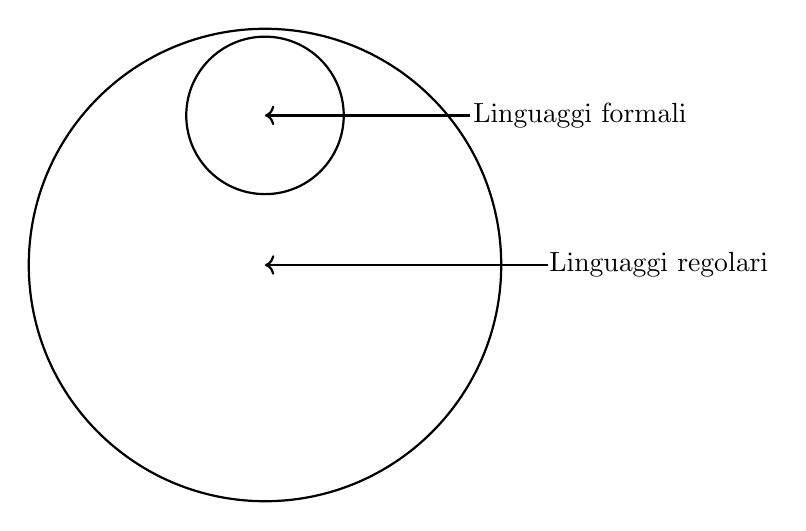
\begin{tikzpicture}
        \draw[thick] (0,0) circle(3);
        \draw[thick] (0,1.9) circle(1);
        \node at (4,1.9) {Linguaggi formali};
        \draw[<-, thick] (0,1.9) -- (2.6,1.9);
    
        \node at (5,0) {Linguaggi regolari};
        \draw[<-, thick] (0,0) -- (3.6,0);
      \end{tikzpicture}
\end{figure}


\begin{figure}[H]
    \centering
    \includegraphics[width=0.6\textwidth]{automa.pdf}
    \caption{Esempio di automa a stati finiti}
\end{figure}
\noindent
Come abbiamo detto in precedenza, una funzione è \textit{calcolabile}
se possiamo pensare ad un algoritmo per calcolarla.
Tra le funzioni calcolabili, ci sono quelle totali, ovvero quelle che terminano per ogni input.
\ex{}
{
    Pensiamo ad una funzione $f \subseteq \mathbb{N} \times \mathbb{N}$,
    la possiamo descrivere come associazione di coppie:
    \[f(0) = 1, f(1) = 1, f(2) = 2, f(3) = 3, f(4) = 5, f(5) = 8, \dots\]
    Tuttavia servirebbe scrivere una quantità infinita di coppie per descrivere la funzione.
    Quindi proviamo a farlo ma stavolta ricorsivamente.
    \[
    \begin{cases}
        f(0) = 1 = f(1)\\
        f(x+2) = f(x+1) + f(x)
    \end{cases}
    \]
}

\subsection{Funzioni e insiemi}

In realtà ci sta un forte legame tra funzioni e insiemi perché per esempio dovessimo prendere una funzione
$f : \mathbb{N} \rightarrow \mathbb{N}$, questa funzione può essere vista come un linguaggio $L_f = \{1^{f(x)} | x \in \mathbb{N}\}$ 
che è l'insieme delle stringhe composte da $f(x)$ simboli 1.
Il nostro linguaggio $\Sigma = \{1\}$ e quindi il linguaggio è un sottoinsieme di $\Sigma^*$.
Il nostro linguaggio ci può dire se un oggetto in input fa parte o no dell'insieme.
Parliamo di \textbf{insiemi} invece che di funzioni
dove gli elementi dell'insieme dipendono dal calcolo della funzione.
\ex{}
{
    Se io dovessi scrivere una funzione costante del tipo $f(x) = 2$.
    In questo caso riconosciamo che il linguaggio $L_f$ è finito perché
    \[L_f = \{1\}\]
    L'unica combinazione possibile è una singola stringa.
    Il linguaggio si dice finito che è sottoinsieme di linguaggi totali.
}
\ex{}
{
    In questo caso la funzione $f(x) = 2x$ è una funzione lineare.
    Ho bisogno di una memoria finita. Mi sposto tra queste informazioni per
    determinare se la stringa in input fa parte o no del linguaggio.
    Questa funzione è anche detta \textbf{regolare}.
}
\ex{}
{
    $f(\sigma) = \sigma_{\text{reverse}}$ quindi per esempio:
    \[f(abc) = cba\]
    Tuttavia per questa funzione non mi basta più una memoria finita ma
    illimitata essendo che non posso sapere a priori quanta memoria abbia bisogno la funzione
    (è sufficiente uno stack).
    Questo tipo di funzione è detta anche \textbf{context free}.
}
\ex{}
{
    Nel caso di $f(x) = x^2$ sappiamo sicuramente
    che possiede un output preciso ma avrei bisogno di una memoria illimitata per rappresentarla.
}

\section{Linguaggi Regolari}

\subsection{Automa a stati finiti determinsitici (DFA)}

Quando parliamo di memoria è facilmente codificabile 
in termini di stati. Dal punto di vista grafico possiamo rappresentarli
come nodi collegati da archi.
Prendiamo per esempio il linguaggio $L_f$ di prima:
\[L_f = \{1^{2n} \; | \; n \in \mathbb{N}\}\]
\[\Sigma = {1}\]

\begin{figure}[H]
    \centering
    \begin{tikzpicture}[node distance = 3cm, on grid, auto]
    
      \node[state, initial, accepting] (q0) {$q_0$};
      \node[state, right of = q0] (q1) {$q_1$};
      \draw (q0) edge[bend left, above] node{1} (q1);
    \draw (q1) edge[bend left, below] node{1} (q0);
    \end{tikzpicture}
  \end{figure}

\dfn{Automa a stati finiti}
{
    \[M = (Q, \Sigma, \delta, q_0, F)\]
    è un automa a stati finiti deterministico dove:
    \begin{itemize}
        \item $Q$ è un insieme finito di stati (ogni stato rappresenta "un informazione")
        \item $\Sigma$ è un alfabeto finito di simboli
        \item $\delta : Q \times \Sigma \rightarrow Q$ è la funzione di transizione (descrive come evolve il
        calcolo a partire dallo stato raggiunto e dal simbolo letto)
        \item $q_0 \in Q$ è lo stato iniziale
        \item $F \subseteq Q$ è l'insieme di stati finali (o di accettazione)
    \end{itemize}
}
\begin{table}[H]
    \centering
    \begin{tabular}{|c|c|c|}
        \hline
        $\Sigma \backslash Q$ & $q_0$ & $q_1$\\
        \hline
        1 & $q_1$ & $q_0$ \\
        \hline
    \end{tabular}
\end{table}
\noindent
Ci sta poi la funzione $\hat{\delta} : Q \times \Sigma^* \rightarrow Q$ che estende la funzione di transizione e descrive
lo stato che raggiungiamo leggendo una sequenza di simboli.
\[
\begin{cases}
    \hat{\delta}(q, \epsilon) = q\\
    \hat{\delta}(q, w a) = \hat{\delta}(\delta(q,w), a)
\end{cases}
\quad w \in \Sigma^*, a \in \Sigma
\]
anche chiamata chiusura transitiva di $\delta$. Quindi mi permette
di calcolare lo stato raggiunto leggendo una stringa di simboli.

\subsection{Come si dimostra che un linguaggio è regolare?}

\ex{}
{
    Prendiamo come esempio il linguaggio:
    \[L = \{\sigma \; | \; \text{ $\sigma$ contiene almeno due 1}\}\]
    \[\Sigma = \{0,1\}\]
    Per esempio:
    \[110, 101, 111, 011, 1001 \in L\]
    \[0, 00, 000, 01, 10, 0000 \notin L\]
    Quindi intuitivamente come possiamo definire l'automa?
    \begin{figure}[H]
        \centering
        \begin{tikzpicture}[->, node distance = 3cm, on grid, auto]
        
          \node[state, initial] (q0) {$q_0$};
          \node[state, right of = q0] (q1) {$q_1$};
          \node[state, accepting, right of = q1] (q2) {$q_2$};


        \draw (q0) edge[bend left, above] node{1} (q1);
        \draw (q0) edge[loop above] node{0} (q0);
        \draw (q1) edge[loop above] node{0} (q1);
        \draw (q1) edge[bend left, above] node{1} (q2);
        \draw (q2) edge[loop above] node{0,1} (q2);
        \end{tikzpicture}
      \end{figure}
    \noindent
    Un linguaggio $L$ è riconosciuto da $M$ (Automa a stati finiti deterministico o DFA)
    se $L = L(M)$ dove $L(M)$ è il linguaggio di $n$ definito come:
    \[L(M) = \{\sigma \in \Sigma^* \; | \; \hat{\delta}(q_0, \sigma) \in F\}\]
    Sono tutte le stringhe che partendo da $q_0$ (stato iniziale) raggiunge uno stato finale.
}
\dfn{}
{
    Per dimostrare che $L$ è regolare dobbiamo costruire $M$ (almeno un $M$) e dimostrare che
    $L(M) = L$.
}
\[L = L(M) \equiv L \subseteq L(M) \text{ e } L(M) \subseteq L\]
\begin{enumerate}
    \item \[L \subseteq L(M) \equiv \sigma . \in L \rightarrow \sigma \in L(M)\]
    \[\sigma \in L \rightarrow \hat{\delta}(q_0, \sigma) \in F\]
    \item 
    \[
    \begin{aligned}
        L(M) \subseteq L &\equiv \sigma \in L(M) \rightarrow \sigma \in L\\
        & \hat{\delta}(q_0, \sigma) \in F \rightarrow \sigma \in L \equiv \\
        &\sigma \notin L \rightarrow \hat{\delta}(q_0, \sigma) \notin F
    \end{aligned}
    \]
\end{enumerate}
Dimostriamo per induzione sulla lunghezza delle stringhe $\sigma \in \Sigma^*$ che
se $\sigma \in L$ allora $\hat{\delta}(q_0, \sigma) \in F$
e $\sigma \notin L$ allora $\hat{\delta}(q_0, \sigma) \notin F$.
\ex{}
{
    \[L = \{\sigma \; | \; \text{ $\sigma$ contiene almeno due 1}\}\]
    \begin{figure}[H]
        \centering
        \begin{tikzpicture}[->, node distance = 3cm, on grid, auto]
        
          \node[state, initial] (q0) {$q_0$};
          \node[state, right of = q0] (q1) {$q_1$};
          \node[state, accepting, right of = q1] (q2) {$q_2$};


        \draw (q0) edge[bend left, above] node{1} (q1);
        \draw (q0) edge[loop above] node{0} (q0);
        \draw (q1) edge[loop above] node{0} (q1);
        \draw (q1) edge[bend left, above] node{1} (q2);
        \draw (q2) edge[loop above] node{0,1} (q2);
        \end{tikzpicture}
      \end{figure}
    \noindent
    Dimostriamo per induzione sulla lunghezza delle stringhe \( \sigma \in \Sigma^* \) 
  che se \( x \in L \) allora \( \hat{\delta}(q_0, x) \in F \) e se \( x \notin L \) allora
  \( \hat{\delta}(q_0, x) \notin F \).

  \vspace{1em}
  \noindent
  \( \left| \sigma  \right| = 0 \) non è \textbf{mai} sufficiente come base, ma
  è eventualmente la base \textbf{solo} per una delle due dimostrazioni. Bisogna
  quindi prendere la lunghezza più piccola che permette di avere sia \( \sigma \in L \) 
  che  \( \sigma \notin L \), in questo caso è \( \left| \sigma  \right| = 2 \).
  Per ogni \( \sigma  \) tale che \( \left| \sigma  \right| < 2 \quad \sigma \notin L \)
  perchè non può contenere due 1 e non è riconosciuta da \( M \) dove il primo stato finale
  è raggiunto leggendo almeno due simboli.
  \[
    \varepsilon \in L \quad \varepsilon \notin L
  \] 
  \begin{itemize}
    \item \textbf{Base}: Controlliamo ogni stringa di lungheezza minima nel linguaggio per
      provare il caso base
      \[
        \begin{cases}
          \sigma &= 11 \in L \; \text{ e } \; \hat{\delta}(q_0, 11) = q_2 \in F \\
          \sigma &= 10 \notin L \; \text{ e } \; \hat{\delta}(q_0, 10) = q_1 \notin F \\
          \sigma &= 01 \notin L \; \text{ e } \; \hat{\delta}(q_0, 01) = q_1 \notin F \\
          \sigma &= 00 \notin L \; \text{ e } \; \hat{\delta}(q_0, 00) = q_0 \notin F
        \end{cases}
      \] 

    \item \textbf{Passo induttivo}: Dimostriamo l'\textbf{ipotesi induttiva}, cioè
      la tesi con un limite fissato:
      \[
        \forall \sigma \in \Sigma^* \;.\; \left| \sigma  \right| \le n \;.\;
        \begin{cases}
          \sigma \in L &\Rightarrow \hat{\delta}(q_0, \sigma) \in F\\
          \sigma \notin L &\Rightarrow \hat{\delta}(q_0, \sigma) \notin F
        \end{cases}
      \] 
      Vogliamo dimostrare se \( \left| \sigma  \right| = n + 1 \) (la successiva stringa
      che posso considerare) allora vale
      \( 
        \begin{cases}
          \sigma \in L \Rightarrow \hat{\delta}(q_0,\sigma) \in F\\
          \sigma \notin L \Rightarrow \hat{\delta}(q_0,\sigma) \notin F
        \end{cases}
      \) 

      \vspace{1em}
      \noindent
      Dimostrazione:
      \[
        \left| \sigma  \right| = n + 1 \to 
          \sigma = \sigma'1 \; \vee \; \sigma = \sigma'0
      \] 
      \begin{itemize}
        \item Supponiamo che \( \sigma  \) appartiene al linguaggio e termini con 1:
          \[
            \sigma \in L \wedge \sigma  = \sigma'1 \to 
          \] 
          \begin{itemize}
            \item Se \( \sigma' \in L \) applico l'ipotesi induttiva:
              \[
                  \hat{\delta}(q_0, \sigma') = q_2\\
              \] 
              \[
                \begin{aligned}
                  \hat{\delta}(q_0, \sigma) &\stackrel{\sigma = \sigma'1}{=}
                  \hat{\delta}(q_0, \sigma'1)\\
                                            &= \delta(\hat{\delta}(q_0, \sigma'), 1)\\
                                            &= \delta(q_2, 1) = q_2 \in F
                \end{aligned}
              \] 

            \item Se \( \sigma' \notin L \) allora \( \sigma' \) contiene esattamente un 1:
              \[
                \hat{\delta}(q_0, \sigma') = q_1
              \] 
              \[
                \hat{\delta}(q_0, \sigma'1) = \delta(q_1, 1) = q_2
              \] 
          \end{itemize}

        \item Supponiamo che \( \sigma  \) appartiene al linguaggio e termini con 0:
          \[
            \sigma \in L \wedge \sigma = \sigma'0
          \] 
          Per definizione di \( L \) abbiamo che
          \[
            \sigma \in L \wedge \sigma = \sigma'0 \Rightarrow \sigma' \in L
          \] 
          Dimostriamo l'ipotesi induttiva:
          \[
            \hat{\delta}(q_0, \sigma') = q_2
          \] 
          allora
          \[
            \begin{aligned}
              \hat{\delta}(q_0, \sigma) &= \hat{\delta}(q_0, \sigma'0)\\
                                        &= \delta(\hat{\delta}(q_0, \sigma'), 0)\\
                                        &= \delta(q_2, 0) = q_2 \in F
            \end{aligned}
          \] 

        \item Supponiamo che \( \sigma  \) non appartiene al linguaggio e termini con 1:
          \[
            \sigma \notin L \wedge  \sigma  = \sigma'1 \text{ (ha esattamente un 1)}
          \] 
          \[
            \Downarrow
          \] 
          \[
            \sigma  \notin L \text{ non ha 1}
          \] 

        \item Supponiamo che \( \sigma  \) non appartiene al linguaggio e termini con 0:
          \[
            \sigma \notin L \wedge  \sigma  = \sigma'0
          \] 
          \[
            \Downarrow
          \] 
          \[
            \sigma' \notin L
          \] 
      \end{itemize}
  \end{itemize}     
}

\ex{Esercizio da esame}
{
\[L = \{\sigma \in \Sigma^* \; | \; \exists n \ge 1 \;  . \; \sigma = 0^n \rightarrow n \ge 2 \}\]
\[\Sigma = \{0,1\}\]
Ovvero ogni sequenza di 0 nella stringa deve essere di lunghezza pari.
Per esempio:
\[101 \notin L, 1111 \in L\]
\[1001 \in L, 000 \notin L, 0000 \in L, 010101 \notin L\]
\begin{figure}[H]
    \centering
    \begin{tikzpicture}[->, node distance = 2cm, on grid, auto]

    \node[state, initial] (q0) {$q_0$};
    \node[state, right of = q0] (q1) {$q_1$};
    \node[state, accepting, right of = q1] (q2) {$q_2$};
    \node[state, above of = q1] (q3) {$q_{\bot}$};

    \draw (q0) edge[bend left, above] node{0} (q1);
    \draw (q0) edge[loop above] node{1} (q0);
    \draw (q1) edge[bend left, above] node{0} (q2);
    \draw (q2) edge[bend left, above] node{0} (q1);
    \draw (q1) edge[bend left, left] node{1} (q3);
    \draw (q3) edge[loop above] node{0,1} (q3);
    \draw (q2) edge[loop above] node{1} (q2);

    \end{tikzpicture}
  \end{figure}
\noindent 
\begin{itemize}
    \item $q_0$: non abbiamo letto 0
    \item $q_1$: rappresenta una sequenza di 0 consecutivi di lunghezza dispari 
    \item $q_2$: sequenza di 0 di lunghezza pari.
\end{itemize}
\[
\text{Tesi: } \begin{cases}
    \sigma \in L \text{ e non contiene 0 } \rightarrow \hat{\delta}(q_0, \sigma) = q_0\\
    \sigma \in L \text{ e contiene 0 } \rightarrow \hat{\delta}(q_0, \sigma) = q_2\\
    \sigma \notin L \text{ e contiene una sequenza finali di 0 } \rightarrow \hat{\delta}(q_0, \sigma) = q_1\\
    \sigma \notin L \text{ e contiene una sequenza dispari di 0 seguiti da un 1 } \rightarrow \hat{\delta}(q_0, \sigma) = q_{\bot}
\end{cases}
\]
}
\ex{}
{
 \[L = \{\sigma \in \Sigma^* \; | \; \exists n \ge 1 \;  . \; \sigma = 0^n \rightarrow n \ge 2 \}\]
\[\Sigma = \{0,1\}\]
Se $\sigma$ non contiene $0$ allora $\sigma \in L$.
\begin{figure}[H]
    \centering
    \begin{tikzpicture}[->, node distance = 2cm, on grid, auto]

    \node[state, initial] (q0) {$q_0$};
    \node[state, right of = q0] (q1) {$q_1$};
    \node[state, accepting, right of = q1] (q2) {$q_2$};
    \node[state, above of = q1] (q3) {$q_{\bot}$};

    \draw (q0) edge[bend left, above] node{0} (q1);
    \draw (q0) edge[loop above] node{1} (q0);
    \draw (q1) edge[bend left, above] node{0} (q2);
    \draw (q1) edge[bend left, left] node{1} (q3);
    \draw (q3) edge[loop above] node{0,1} (q3);
    \draw (q2) edge[loop above] node{0} (q2);
    \draw (q2) edge[bend left, below] node{1} (q0);

    \end{tikzpicture}
  \end{figure}   
  \noindent
  \begin{itemize}
    \item $q_0$: non contiene 0 oppure tutte le sequenze di 0 sono lunghe almeno 2.
    \item $q_1$: esattamente uno 0.
    \item $q_2$: almeno due 0.
  \end{itemize}
  \[\text{Tesi: } 
  \begin{cases}
    \sigma \in L \text{ e } \sigma = \sigma'1 \rightarrow \hat{\delta}(q_0, \sigma) = q_0\\
    \sigma \in L \text{ e } \sigma = \sigma'0 \rightarrow \hat{\delta}(q_0, \sigma) = q_2\\
    \sigma \notin L \text{ e } \sigma = \sigma'0 \text{ dove l'ultima seq di 0 è esattamente lunga 1} \rightarrow \hat{\delta}(q_0, \sigma) = q_1\\
    \sigma \notin L \text{ e } \sigma \text{ contiene una sequenza lunga 1 di 0} \rightarrow \hat{\delta}(q_0, \sigma) = q_{\bot}
  \end{cases}\]
}

\subsection{Automi a stati finiti non deterministici (NFA)}

\dfn{}
{
    Un automa a stati finiti non deterministico è una 5-upla:
    \[N = (Q, \Sigma, \delta, q_0, F)\]
    dove:
    \begin{itemize}
        \item $Q$ è un insieme finito di stati
        \item $\Sigma$ è un alfabeto finito di simboli
        \item $q_0 \in Q$ è lo stato iniziale
        \item $F \subseteq Q$ è l'insieme di stati finali (o di accettazione)
        \item $\delta : Q \times \Sigma \rightarrow \mathcal{P}(Q)$ è la funzione di transizione dove 
        per ogni coppia di stato-simbolo ho un insieme di stati potenzialmente raggiungibili.
    \end{itemize}
}
\begin{figure}[H]
    \centering
    \begin{tikzpicture}[->, node distance = 2cm, on grid, auto]

    \node[state, initial] (q0) {$q_0$};
    \node[state, above right of = q0] (q1) {$q_1$};
    \node[state, below right of=q0] (q2) {$q_2$};

    \draw (q0) edge[bend left, above] node{a} (q1);
    \draw (q0) edge[bend right, below] node{a} (q2);

    \end{tikzpicture}
  \end{figure}   
  \[\delta(q_0, a) = \{q_1, q_2\} \subseteq Q\]
  \[ \varnothing \in \mathcal{P}(Q)\]
  \begin{itemize}
    \item È possibile che non esistano coppie associate al vuoto
    \item Non è obbligatorio avere un arco uscente per ogni simbolo di $\Sigma$.
  \end{itemize}
    \noindent
    Definiamo $\hat{\delta}: \hat{\delta}: Q \times \Sigma^* \rightarrow \mathcal{P}(Q)$
    \[
    \begin{cases}
        \hat{\delta}(q, \epsilon) = \{q\}\\
        \hat{\delta}(q, w a) = \bigcup_{p \in \hat{\delta}(q,w)} \delta(p, a)
    \end{cases}
    \]
    Linguaggio riconosciuto:
    \[L(N) = \{\sigma \in \Sigma^* \; | \; \hat{\delta}(q_0, \sigma) \cap F \neq \varnothing \}\]
    \thm{Teorema di Rabin-Scott}
    {
        Se abbiamo $N = (Q, \Sigma, \delta, q_0, F)$ un NFA allora esiste 
        $M$ DFA tale che $L(N) = L(M)$.
    }
    Quindi se $M$ DFA allora $N$ è un particolare $NFA$.
    \begin{proof}
        Preso $N = (Q, \Sigma, \delta, q_0, F)$ costruiamo $M = (Q', \Sigma, \delta', q_0', F')$ dove:
        \[Q' = \mathcal{P}(Q)\]
        \[Q = \{q_0, q_1, q_2\}\]
        \[Q' = \{\varnothing, 
        \{q_0\}, \{q_1\},
        \{q_2\}, \{q_0, q_1\}, \{q_0, q_2\},
        \{q_1, q_2\}, \{q_0, q_1, q_2\}\}\]
        \[q_0' = \{q_0\}\]
        \[F = \{q_2\}\]
        \[F' = \{\underbrace{P \subseteq Q}_{P \in \mathcal{P}(Q)} \; | \; P \cap F \neq \varnothing\}\]
        \[F' = \{\{q_2\}, \{q_1q_2\}, 
        \{q_0q_2\},\{q_0q_1q_2\}
        \}\]
        \[\delta'(P, a) = \bigcup_{q \in P} \delta(q, a) \in \mathcal{P}(Q)\]
        \[
        \begin{aligned}
            \delta'(q_5',1) &= \delta(q_1,1) \cup \delta(q_2,1)\\
            &= \{q_0, q_2\} \cup \{q_0, q_1, q_2\}\\
            &= \{q_0, q_1, q_2\}
        \end{aligned}
        \]
        Dimostriamo:
        \begin{enumerate}
            \item  $\hat{\delta}'{q_0', \sigma} = \hat{\delta}(q_0, \sigma)$ 
            \item $\sigma \in L(N) \text{ sse } \sigma \in L(M)$
        \end{enumerate}
        \begin{enumerate}
            \item Per induzione su $|\sigma|$:\\
            Se $\sigma = \epsilon$ allora: $\hat{\delta}'(q_0', \epsilon) = q_0' = \{q_0\} = \hat{\delta}(q_0, \epsilon)$ per le definizioni.\\
            Se $\sigma = \sigma'a$: $\hat{\delta}'({q_0', \sigma'a}) = \hat{\delta}(\hat{\delta}'(q_0, \sigma'), a)$. Per ipotesi induttiva:
            \[\hat{\delta}'(q_0', \sigma') = \hat{\delta}(q_0, \sigma')\]
            \item $\sigma \in L(N) \text{ sse } \sigma \in L(M)$
            \[
            \begin{aligned}
              \sigma \in L(N) &\Leftrightarrow \hat{\delta}(q_0, \sigma) \cap F \neq \varnothing\\
                &\Leftrightarrow \hat{\delta}'(q_0', \sigma) \cap F \neq \varnothing\\
                &\Leftrightarrow \hat{\delta}'(q_0', \sigma) \in F'\\
                &\Leftrightarrow \sigma \in L(M) \text{ def. linguaggio accettato in DFA}  \quad \square
            \end{aligned} 
            \]
        \end{enumerate}
    \end{proof}
\noindent
Una volta aver raggiunto un risultato di automa a stati finiti deterministico non è
detto che sia il migliore che possiamo trovare. Possiamo \textit{eliminare gli stati non raggiungibili} e ottenere un
automa equivalente più piccolo (\textbf{DFA minimo}).

\subsubsection{Automi non deterministici con $\varepsilon$-transizioni ($\varepsilon$-NFA)}

Gli $\varepsilon$-NFA sono una variante degli NFA in cui possiamo cambiare stato 
senza leggere simboli.

\[q_1 \stackrel{\varepsilon}{\rightarrow} q_2 \]

\dfn{}
{
    Un $\varepsilon$-NFA è una 5-upla:
    \[N = (Q, \Sigma, \delta, q_0, F)\]
    dove:
    \begin{itemize}
        \item $Q$ è un insieme finito di stati
        \item $\Sigma$ è un alfabeto finito di simboli
        \item $q_0 \in Q$ è lo stato iniziale
        \item $F \subseteq Q$ è l'insieme di stati finali (o di accettazione)
        \item $\delta : Q \times (\Sigma \cup \{\varepsilon\}) \rightarrow \mathcal{P}(Q)$ è la funzione di transizione dove 
        per ogni coppia di stato-simbolo ho un insieme di stati potenzialmente raggiungibili.
        La $\varepsilon$ mi dice che possiamo cambiare stato senza leggere simboli.
    \end{itemize}
}
\noindent
Per esempio:
\begin{figure}[H]
  \centering
  \begin{tikzpicture}[->, node distance = 2cm, on grid, auto]

  \node[state, initial] (q0) {$q_0$};
  \node[state, right of = q0] (q1) {$q_1$};
  \node[state, right of=q1] (q2) {$q_2$};

  \draw (q0) edge[above] node{a} (q1);
  \draw (q1) edge[above] node{$\varepsilon$} (q2);
  \draw (q0) edge[bend left, above] node{a} (q1);
  \draw (q0) edge[bend left, above] node{a} (q2);
  \end{tikzpicture}
\end{figure}  
\noindent 
Definiamo ora:
\[\hat{\delta}: Q \times \Sigma^* \rightarrow \mathcal{P}(Q)\]

\[\varepsilon-\text{closure}: Q \rightarrow \mathcal{P}(Q)\]
La $\varepsilon$-closure$(q)$ di uno stato $q$ è l'insieme di stati raggiungibili da $q$
seguendo archi etichettati con $\varepsilon$.
\[\varepsilon-\text{closure}: \mathcal{P}(Q) \rightarrow \mathcal{P}(Q)\]
\[
  \begin{cases}
    \hat{\delta} (q, \epsilon) = \varepsilon\text{-closure}(q)\\
    \hat{\delta} (q, w a) = \varepsilon\text{-closure}\left(\bigcup_{p \in \hat{\delta}(q,w)} \delta(p, a)\right)
  \end{cases}
\]
\ex{}
{
  La $\varepsilon$-closure di $q'$ nell'automa sopra è:
  \[
  \varepsilon\text{-closure}(q') = \{q', q''\}
  \]
}
Il riconoscimento di  un linguaggio è analogo a quello di un NFA:
\[L(N) = \{\sigma \in \Sigma^* \; | \; \hat{\delta}(q_0, \sigma) \cap F \neq \varnothing\}\]
\thm{}
{
  Sia $N = (Q, \Sigma, \delta, q_0, F)$ un $\varepsilon$-NFA.
  Allora esiste un NFA $N'$ tale che $L(N) = L(N')$.
}
\noindent
Ciò vuol dire che l'insieme dei linguaggi riconosciuti da $\varepsilon$-NFA 
coincide con quello degli NFA, che a sua volta coincide con i linguaggi regolari.
Prendiamo $N = (Q, \Sigma, \delta, q_0, F)$ un $\varepsilon$-NFA.
Costruiamo NFA $N' = (Q', \Sigma', \delta, q_0', F')$ dove $\delta'(q,a) = \hat{\delta}(q,a)$
e $F' = \begin{cases}
  F \cup \{q_0\} & \text{se } \varepsilon\text{-closure}(q_0) \cap  F \neq \varnothing\\
  F & \text{altrimenti}
\end{cases}$.

\subsection{Espressioni Regolari}

Le espressioni regolari sono un modo compatto per rappresentare i linguaggi.
Le opreazioni che si possono fare sono:
\begin{itemize}
  \item Unione: Siano $L_1, L_2 \subseteq \Sigma^*$ linguaggi : $L_1 \cup L_2 = \{\sigma \; | \; \sigma \in L_1 \text{ oppure } \sigma \in L_2\}$
  \item Concatenazione: Siano $L_1, L_2 \subseteq \Sigma^*$ linguaggi : $L_1 \cdot L_2 = \{\sigma_1 \sigma_2 \; | \; \sigma_1 \in L_1, \sigma_2 \in L_2\}$ che permette
  la concatenazione di tutte le stringhe di $L_1$ con tutte le stringhe di $L_2$.
  \item Stella di Kleene: Sia $L \subseteq \Sigma^*$ un linguaggio : $L^* = \bigcup_{n \in \mathbb{N}} L^n$ dove 
  $L^n$ è la concatenazione di $L$ con sè stesso $n$ volte.
  \[
  \begin{cases}
    L^0 = \{\varepsilon\}\\
    L^{n+1} = L^n \cdot L
  \end{cases}
  \]
  \[L = \{000, 111\}\]
  \[
  \begin{aligned}
    L^0 &= \{\varepsilon\}\\
    L^1 &= \{000, 111\} = L\\
    L^2 &= \{000000, 000111, 111000, 111111\}\\
    L^3 &= \{000000000, 000000111, 000111000, 000111111, 111000000, 
    \\&111000111, 111111000, 111111111\}\\
    &\vdots\\
    L^* &= \bigcup_{n \in \mathbb{N}} L^n
  \end{aligned}
  \]
  \[L^+ = \bigcup_{n \ge 0} L^n\]
\end{itemize}

\dfn{}
{
  $\Sigma$ alfabeto, definiamo per induzione:
  \begin{itemize}
    \item \textbf{Caso base:}
  \begin{itemize}
    \item $\varnothing \subseteq \Sigma^*$ è espressione regolare che rappresenta il linguaggio vuoto.
    \item $\varepsilon$ è espressione regolare che rappresenta il linguaggio $\{\varepsilon\} \subseteq \Sigma^*$.
    \item $a \in \Sigma$ è espressione regolare che rappresenta il linguaggio $\{a\} \subseteq \Sigma^*$. 
  \end{itemize}
  \item \textbf{Passo induttivo:}
  \begin{itemize}
    \item $r, s$ sono espressioni regolari che rappresentono il linguaggio $R \subseteq \Sigma^\alpha$ e $S \subseteq \Sigma^*$ rispettivamente.
    \begin{itemize}
      \item $(r)+(s)$ è espressione regolare che rappresenta il linguaggio $R \cup S$.
      \item $(r)(s)$ è espressione regolare che rappresenta il linguaggio $R \cdot S$.
      \item $(r)^*$ è espressione regolare che rappresenta il linguaggio $R^*$.
    \end{itemize}
  \end{itemize}
\end{itemize}
}
\ex{}
{
  Prendiamo come esempio la seguente espressione:
  \[1^* + 0^* + (10)^*\]
  equivale:
  \[\{1^n \; | \; n \in \mathbb{N}\} \cup \{0^n \; | \; n \in \mathbb{N}\} \cup \{(10)^n \; | \; n \in \mathbb{N}\}\]
  Un'altra equivalenza interessante è:
  \[L = {000,111} \rightarrow (000 + 111)\]
  \[L^* = (000 + 111)^*\]
}


\thm{Teorema di equivalenza}
{
  Dato $M$ DFA $(Q, \Sigma, \delta, q_0, F)$ allora 
  esiste $r$ espressione regolare t.c $L(N) = L(r)$.
  \[\text{L regolare} \stackrel{def}{\Leftrightarrow} \exists \underbrace{M \; DFA}_{L(n) = L} \stackrel{thm}{\rightarrow} \exists r \in ER \; | \; L(r) = L\]
}
\thm{}
{
  Data $r$ espressione regolare (ER) allora esiste un $\varepsilon$-NFA $M$ tale che $L(r) = L(N)$.
  \begin{itemize}
    \item $\varepsilon \leadsto q_0, L(N) = \{\varepsilon\}$
    \item $\varnothing \leadsto q_0, q_1, L(N) = \varnothing$
    \item $a \leadsto q_0 \rightarrow q_1, L(N) = \{a\}$ 
    \item $r,s$ espressioni regolari per ipotesi induttiva
    $\exists N_1 . L(n_1) = L(r)$ e $\exists N_2 . L(n_2) = L(s)$.
  \end{itemize}
}
\[r \; ER \Rightarrow M \; \varepsilon\text{-closure} \Longleftrightarrow M' \text{ DFA} \Longleftrightarrow L(M') \text{ è regolare}\]
\ex{}
{
  \[L = \{\sigma \in \Sigma^* \; | \; \sigma \text{ contiene almeno due 1}\}\]
  per dimostrare che è regolare si costruisce il DFA $M$ e si dimostra ceh $L = L(M)$.
  \[r = 0^*10^*10^*\]
  dove $r$ non dimostra che $L$ è regolare, perché dovremmo dimostrare $L = L(r)$.
  $L(r)$ è sicuramente regolare ma dobbiamo \textbf{comunque} dimostrare l'uguaglianza insiemistica $L = L(r)$.
}

\subsection{Proprietà di LR (linguaggi regolari)}

\subsubsection{Proprietà di chiusura}

Rispetto a quali operazioni due linguaggi regolari sono chiusi?
Questa proprietà è utile perché a volte mi serve studiare un linguaggio complesso
come intersezioni di linguaggi più semplici.
Operazioni: $*, \cup, \cdot, \cap, \hat{}$.
\thm{}
{
  I linguaggi sono chiusi rispetto a stella di Kleene, unione (finita) e concatenazione.
}
\noindent
Quindi
\[L_1, L_2 \text{ reg}\]
\[L^* \text{ è reg. } L_1 \cup L_2 \text{ reg} \quad L_1L_2 \text{ è regolare} \]
\[\underbrace{a^3}_{\text{reg. finito}} \cdot \{b^nc^m \; | \; n,m \in \mathbb{N}\}\]
\thm{}
{
  I linguaggi regolari sono chiusi rispetto alla complementazione.
}

\begin{figure}[H]
  \centering
  \begin{tikzpicture}[->, node distance = 3cm, on grid, auto]
  
    \node[state, initial] (q0) {$q_0$};
    \node[state, right of = q0] (q1) {$q_1$};
    \node[state, accepting, right of = q1] (q2) {$q_2$};


  \draw (q0) edge[bend left, above] node{1} (q1);
  \draw (q0) edge[loop above] node{0} (q0);
  \draw (q1) edge[loop above] node{0} (q1);
  \draw (q1) edge[bend left, above] node{1} (q2);
  \draw (q2) edge[loop above] node{0,1} (q2);
  \end{tikzpicture}
\end{figure}
\begin{figure}[H]
  \centering
  \begin{tikzpicture}[->, node distance = 3cm, on grid, auto]
  
    \node[state, accepting] (q0) {$q_0$};
    \node[state, accepting, right of = q0] (q1) {$q_1$};
    \node[state, initial, right of = q1] (q2) {$q_2$};


  \draw (q0) edge[bend left, above] node{1} (q1);
  \draw (q0) edge[loop above] node{0} (q0);
  \draw (q1) edge[loop above] node{0} (q1);
  \draw (q1) edge[bend left, above] node{1} (q2);
  \draw (q2) edge[loop above] node{0,1} (q2);
  \end{tikzpicture}
\end{figure}
\noindent
L'automa sopra disegnato riconosce il complemento.
\[L_1 \cap L_2 = \overline{\overline{L_1} \cup \overline{L_2}}\]
per le leggi di Morgan, i linguaggi regolari sono chiusi per intersezione (finita).


\subsubsection{Proprietà di decidibilità}

L'insieme di stringhe accettate da un DFA (linguaggio regolare) 
DFA con $M$ stati con $n$ stati.
\begin{enumerate}
  \item $L(M)$ è $\neq \varnothing$ sse accetta almeno una stringa di lunghezza $\le n$.
  \item $L(M)$ è infinito se accetta almeno una stringa lunga $l$ con $n \le l \le 2n$.
  \item $L(M_1) = L(M_2)$ cazzo piccolissimooo... 8======D
\end{enumerate}

\subsubsection{Esistenza dell'automa minimo}

Fornisce strategie per costruire un automa minimo. Sia $R$ relazione su $\Sigma: R \subseteq \Sigma \times \Sigma$.
  $R$ è una relazione di equivalenza se:
  \begin{itemize}
    \item Riflessiva: $\forall a \in \Sigma . aRa$
    \item Simmetrica: $\forall a,b \in \Sigma . aRb \Rightarrow bRa$
    \item Transitiva: $\forall a,b,c \in \Sigma . aRb \wedge bRc \Rightarrow aRc$
  \end{itemize}
  Una relazione di equivalenza induce una partizione.
  $R \subseteq S \times S$ induce una partizione di $S$ dove $S_i$ sono una partizione di $S$ se 
  \[S = S_1 \cup S_2 \cup \dots \cup S_n\]
  e 
  \begin{itemize}
    \item $\forall i,j \; S_i \cap S_j = \varnothing$
    \item $\forall a,b \in S_i . aRb$
    \item $\forall a \in S \, \forall b \in S_j . \neg(aRb)$
  \end{itemize}
  $S_i$ sono detti classi di equivalenza di $R$:
  \[a \in R \Rightarrow [a]_R = \{b \; | \; aRb\} \text{ classe di equivalenza di a}\]
  \[cRa \Rightarrow [a]_R \equiv [c]_R\]

\noindent
Torniamo ora ai linguaggi regolari.
Consideriamo un linguaggio $L \subseteq \Sigma^*$.
Possiamo definire $R_L \subseteq \Sigma^* \times \Sigma^*$ come:
\[x,y \in \Sigma^* \quad xR_Ly \text{ sse } \forall z \in \Sigma^* . xz \text { sse } yz \in L\]
Quello che diciamo quindi è che due stringhe sono in relazione se per ogni possibile estensione $z$
la loro appartenenza a $L$ è la stessa.
\dfn{Classe di equivalenza definita per gli automi}
{
  Consideriamo $M = (Q, \Sigma, \delta, q_0, F)$ un DFA. Possiamo definire
  $R_M \subseteq \Sigma^* \times \Sigma^*$ come:
  \[x,y \in \Sigma^* . xR_my \Longleftrightarrow \hat{\delta}(q_0, x) = \hat{\delta}(q_0,y)\]
  \begin{figure}[H]
    \centering
    \begin{tikzpicture}[->, node distance = 3cm, on grid, auto]
    
      \node[state] (q0) {$q_0$};
      \node[state, right of = q0] (q1) {$q_1$};
      
    \draw (q0) edge[bend left, above] node{x} (q1);
    \draw (q0) edge[bend right, below] node{y} (q1);

    \end{tikzpicture}
  \end{figure}
  \noindent
  Allora \textbf{$R_L$ e $R_M$ sono relazioni di equivalenza.}
}
\dfn{Relazione invariante destra}
{
  Una relazione di equivalenza $R$ su $\Sigma^*$ è invariante a destra se:
  \[\forall x,y,z \in \Sigma^* \quad xRy \Rightarrow xzRyz\]
  Quindi essere in relazione è invariante rispetto all'estensione della stringa verso destra.
  \textbf{$R_L$ e $R_M$ sono relazioni invarianti destra.}
}
\dfn{Raffinamento}
{
  Siano $R$ e $S$ due relazioni di equivalenza su $\Sigma^*$.
  Diciamo che $R$ raffina $S$ se:
  \[\forall x,y \in \Sigma^* \quad xRy \Rightarrow xSy\]
  Quindi ogni classe di equivalenza di $R$ è contenuta in una classe di equivalenza di $S$.
  Il numero di classi di equivalenza di $R$ è maggiore del numero di classi di equivalenza di $S$.
}
\dfn{}
{
  Dato un DFA $M = (Q, \Sigma, \delta, q_0, F)$ ogni
  stato definisce un linguaggio.
  \[q \in Q : L_q = \{x \in \Sigma^* \; | \; \hat{\delta}(q_0, x) = q\}\]
}
\noindent
$R$ si dice di indice finito se il numero di classi di equivalenza indotte è finito.

\thm{Teorema di Nyhill-Nerode}
{
  I seguenti enunciati sono equivalenti:
  \begin{enumerate}
    \item $L \subseteq \Sigma^*$ è regolare ovvero esiste un DFA $M$ t.c. $L(M) = L$.
    \item $L$ è l'unione di classi di equivalenza indotte da una relazione di equivalenza $R$ 
    invariante destra con indice finito.
    \item $R_L$ è di indice finito.
  \end{enumerate}
}
Dimostriamo che:
\[(1) \stackrel{R_m}{\Longrightarrow} (2) \stackrel{R \text{ raffina } R_L}{\Longrightarrow} (3) \stackrel{\text{costruisce } M}{\Longrightarrow} (1)\]
\begin{proof}
  $(1) \Rightarrow (2)$\\
  Ipotesi: $L$ linguaggio riconosciuto da $M = (Q, \Sigma, \delta, q_0, F)$ DFA. 
  \[L = L(M)\]
  Tesi: $\exists R$ relazione di equivalenza invariante destra di indice finito t.c. $L$ è l'unione di classi di equivalenza di $R$. 
  Prendiamo $R = R_M \quad xR_my$ sse $\hat{\delta}(q_0, x) = \hat{\delta}(q_0,y)$.
  \begin{enumerate}
    \item Il numero di classi di equivalenza di $R_M$ è uguale al numero di stati $|Q|$ ma 
    per definizione $Q$ è finito quindi $R_M$ è di indice finito.
    \item $R_M$ è invariante destra:
    \[
    \begin{aligned}
      L = L(M) &= \{x \in \Sigma^* \; | \; \hat{\delta}(q_0, x) \in F\}\\
      &= \{x \in \Sigma^* \; | \; \hat{\delta}(q_0,x) = q \wedge q \in F\}\\
      &= \bigcup_{\substack{q \in F}} \{x \; | \; \hat{\delta}(q_0, x) = q\}\\
      &= \bigcup_{\substack{q \in F}} L_q \text{ dove } L_q \text{ è la classe di equivalenza di } R_M
    \end{aligned}
    \]
    Quindi $L$ è l'unione di classi di equivalenza di $R_M$.
  \end{enumerate}
\end{proof}
\begin{proof}
 $(2) \Rightarrow (3)$\\
 Ipotesi: $L$ è l'unione di classi di equivalenza indotte da una relazione di equivalenza $R$ di indice finito.\\
 Tesi: $R_L$ è di indice finito.
 Possiamo dimostrare che $R$ raffina $R_L$. Perché se fosse così allora il numero di classi di $R$ 
sarebbe maggiore del numero di classi di $R_L$. Quindi se il numero di classi di $R$ è finito allora sicuramente
lo sarà anche $R_L$.
Per dimostrare $R$ raffinamento di $R_L$ dobbiamo dimostrare che $\forall x,y \in \Sigma^* \quad xRy \Rightarrow xR_Ly$.
In maniera equivalente:
\[y \in [x]_R \Rightarrow y \in [x]_{R_L} \equiv [x]_R \subseteq [x]_{R_L}\]
Prendiamo $xRy$ sapendo che $R$ è invariante destra.
\[
\forall z \in \Sigma^* \quad xRy \Rightarrow xzRyz
\]
Quindi se $L$ è l'unione di classi di equivalenza di $R$:
\[xRy \quad x \in L \text{ sse } y \in L\]
\[[x]_R \subseteq L \text{ oppure } [x]_R \text{ fuori da } L\]
Quindi:
\[
\begin{aligned}
  xRy &\Longrightarrow x \in L \Longleftrightarrow y \in L\\
  &\Longrightarrow \forall z \; . \; xzRyz \Longrightarrow xz \in L \Longleftrightarrow yz \in L\\
  &\stackrel{\text{def } R_L}{\Longrightarrow} xR_Ly
\end{aligned}
\]
Queste dimostrazioni dato $M$ generico, $R_M$ è un raffinamento
di $R_L$.
\end{proof}
\begin{proof}
  $(3) \Rightarrow (1)$\\
  Ipotesi: $R_L$ è di indice finito.\\
  Tesi: $L$ è riconosciuto da un DFA $M$.\\
  Costruiamo $M$:
  \begin{itemize}
    \item  $Q = \{[x]_{R_L} \; | \; x \in \Sigma^*\}$ è l'insieme delle classi di equivalenza di $R_L$ (sono finite)
    \item $\Sigma = \text{quello di } L$
    \item $q_0 = [\varepsilon]_{R_L}$
    \item $F = \{[x]_{R_L} \; | \; x \in L\}$
    \item $\delta(q, a) = \delta([x]_{R_L}, a) = [xa]_{R_L}$ questo è vero perché $R_L$ è invariante destra.
    $\delta$ è una buona definizione perché indipendente dall'elemento che rappresenta la classe.
  \end{itemize}
  Ora dobbiamo dimostrare che $L = L(M)$.
  Dimostrare per induzione che $\hat{\delta}([x], y) = [xy]$:
  \[\hat{\delta}(q_0,x) = \hat{\delta}([\varepsilon]_{R_L},x) = [x]_{R_L}\]
  \[
  \begin{aligned}
    x \in L(M) &\text{ sse } \hat{\delta}(q_0,x) \in F\\
    &\text{ sse } \hat{\delta}([\varepsilon]_{R_L},x) \in F\\
    &\text{ sse } [x]_{R_L} \in F\\
    &\text{ sse } x \in L \quad \square
  \end{aligned}
  \]
  Quindi $L(M) = L$.
\end{proof}
\thm{}
{
  Dato $L$ esiste $M$ DFA t.c. $L(M) = L$ e $M$ ha il numero minimo di stati (quello costruito da $R_L$).
}

\subsubsection{Pumping Lemma per linguaggi regolari}

Questo risultato è importante perché fornisce una condizione $\pi$ necessaria alla regolarità.
\[L \text{ regolare} \Longrightarrow \pi\]
Questa forma si può riscrivere come:
\[\neg \pi \Longrightarrow L \text{ non è regolare}\]

\thm{Pumping Lemma}
{
  Sia $L \subseteq \Sigma^*$ un linguaggio regolare.
  Allora esiste  $k \in \mathbb{N}$ t.c. per ogni stringa $s \in L$ con $|s| \ge k$ 
  può essere scritta come:
  \[s = uvw\]
  con:
  \begin{itemize}
    \item $|v| > 0$
    \item $|uv| \le k$
    \item $\forall i \in \mathbb{N} \; . \;  uv^iw \in L$
  \end{itemize}
}

\begin{proof}
$L$ regolare se esiste $M$ DFA t.c $L = L(M)$ dove $ M = (Q, \Sigma, \delta, q_0, F)$.
\[|Q| = n \in \mathbb{N}, k = n \quad z \in L \; t.c. \; |z| \ge k\]
\[z = a_1a_2 \dots a_m \quad m \ge k\]

\begin{figure}[H]
  \centering
  \begin{tikzpicture}[->, node distance = 2.5cm, on grid, auto]
  
    \node[state] (q0) {$q_0$};
    \node[state, right of = q0] (q1) {$q_1$};
    \node[state, right of = q1] (q2) {$q_2$};
    \node (dots) {$\ldots$};
    \node[state, right of = q2] (qm) {$q_{m+1}$};
    
  \draw (q0) edge[ above] node{$a_1$} (q1);
  \draw (q1) edge [above] node{$a_2$} (q2);
  \draw (q2) edge[above, dotted] node{$a_m$} (qm);

  \end{tikzpicture}
\end{figure}
\noindent
Per leggere $m$ simboli si attraverso $m+1$ stati. 
Ma $m \ge n \Rightarrow$ attraverso almeno $n+1$ stati. Attraversiamo 
più stati di quelli in $Q$ ovvero almeno uno stato è ripetuto nel riconoscimento di $z$. 
Suppiniamo $\bar{q} \in Q$ sia il primo stato leggendo $z$ che
viene ripetuto, in cui si torniamo per riconoscere $z$. 
\begin{figure}[H]
  \centering
  \begin{tikzpicture}[->, node distance = 3cm, on grid, auto]
  
    \node[state] (q0) {$q_0$};
    \node[state, right of = q0] (qb) {$\bar{q}$};
    \node[state, right of = qb] (qm) {$q_{m+1}$};
    
  \draw (q0) edge[ above] node{$a_1$} (qb);
  \draw (qb) edge [loop above] node{$a_i \dots a_j$} ();
  \draw (qb) edge[above] node{$a_{j+1} \dots a_m$} (qm);

  \end{tikzpicture}
\end{figure}
\noindent
Non ci sono stati ripetuti perché $\bar{q}$ è il primo per costruzione.
$u$ da $q_0$ a $\bar{q}$, $v$ da $\bar{q}$ a $\bar{q}$, $w$ da $\bar{q}$ a $q_{m}$ finale.
Questa suddivisione è accettabile per il lemma?
\begin{itemize}
  \item $|uv| \le k$ 
  \begin{figure}[H]
    \centering
    \begin{tikzpicture}[->, node distance = 2.5cm, on grid, auto]
    
      \node[state] (q0) {$q_0$};
      \node[state, right of = q0] (q1) {$q_1$};
      \node[state, right of = q1] (q2) {$q_2$};
      \node (dots) {$\ldots$};
      \node[state, right of = q2, accepting] (qm) {$q_{m+1}$};
      
    \draw (q0) edge[ above] node{$a_1$} (q1);
    \draw (q1) edge [above] node{$a_2$} (q2);
    \draw (q2) edge[above, dotted] node{$a_2 \dots a_m$} (qm);
    \draw (qm) edge[loop above] node{$a_{n+1} = a_m$} (qm);
    
  
    \end{tikzpicture}
  \end{figure}
  \noindent
  Per arrivare allo stato finale $q_m$ si attraversano $m-1$ simboli.
  \[Q = \{q_0, q_1, \dots, q_{m-1}\} \rightarrow |Q| = m\]
  \item $|v| > 0$ perché altrimenti non ci sarebbe stato ripetuto, sappiamo 
  che per forza di cose almeno un arco deve uscire dallo stato e ritornare nello stesso stato.
  \item $\forall i \in \mathbb{N} \; . \; uv^iw \in L$ 
  
  \begin{figure}[H]
    \centering
    \begin{tikzpicture}[->, node distance = 3cm, on grid, auto]
    
      \node[state] (q0) {$q_0$};
      \node[state, right of = q0] (q1) {$q_1$};
      \node[state, right of = q1] (qb) {$\bar{q}$};
      \node[state, right of = qb, accepting] (qm) {$q_{m+1}$};
      
    \draw (q0) edge[ above] node{$a_1$} (q1);
    \draw (q1) edge [above, dotted] node{$a_2$} (qb);
    \draw (qb) edge[loop above] node{$v^i$} ();
    \draw (qb) edge[above, dotted] node{$w$} (qm);  
    \end{tikzpicture}
  \end{figure}
  \noindent
  perché essendo $v$ un ciclo, ripeterlo $i$ volte mi riporta sempre nello stato $\bar{q}$. $\square$
\end{itemize}
\end{proof}
\noindent
Ora proviamo a negare il pumping lemma per dimostrare che un linguaggio non è regolare.
\begin{itemize}
  \item $\exists k \leadsto \forall k$ quindi la dimostrazione non deve imporre vincoli
  su $k$.
  \item $\forall z \leadsto \exists z \in L \; . \; |z| \ge k$ quindi costruiamo noi la $z \in L$ di lunghezza $k$.
  \item $\exists uvw = z \leadsto \forall uvw = z$ quindi dobbiamo dimostrare che per ogni possibile suddivisione ($|v| > 0, |uv| \le k$)
  \item $\forall i \in \mathbb{N} \leadsto \exists i \in \mathbb{N}$ quindi dobbiamo trovare un $i$ che rispetti la condizione $uv^iw \notin L$.
\end{itemize}
\ex{}
{
  Consideriamo il seguente linguaggio:
  \[L = \{0^n1^n \; | \; n \in \mathbb{N}\}\]
  Dimostriamo che $L$ non è regolare tramite il pumping lemma.
  \[\forall k \in \mathbb{N} \; . \; \exists z \in L \; |z| \ge k \quad \forall uvw = z \; \; |uv| \le k \; \; |v| > 0 \quad \exists i \; . \; uv^iw \notin L\]
  Fissiamo $k \in \mathbb{N}$ ($k$ non deve avere nessun vincolo):
  \[z = 0^k1^k \in L \quad |z| \ge k\]
  \textbf{Condizioni di appartenenza} a $L$:
  \[0^a1^b \in L \text{ sse } a = b\]
  Gli 0 e gli 1 devono avere cardinalità uguale.
  Quindi una singola suddivisione che va bene posso solo prendere 
  $uv \in 0^k$ perché per ipotesi $|uv| \le k$.
  Andiamo ora a definire \[z_i = uv^iw = 0^{k+(i-1)|v|}1^k\]
  Prendiamo per esempio $i = 0$:
  \[0^{k+(0-1)|v|}1^k = 0^{k - |v|}1^k\]
  e quindi abbiamo effettivamente tolto l'interezza di $v$.\\
  Per $i = 1$:
  \[0^{k+(1-1)|v|}1^k = 0^k1^k\]
  Per $i = 3$ (ripete tre volte $v$):
  \[0^{k+(3-1)|v|}1^k = 0^{k + 2|v|}1^k \]
  \[z_i = 0^{k+(i-1)|v|}1^k\]
  In questo caso, dobbiamo rompere la condizione di appartenenza per cui $a \neq b$.
  Basterebbe ripetere $v$ almeno una volta, quindi prendiamo $i = 2$:
  \[z_2 = 0^{k+(2-1)|v|}1^k = 0^{k + |v|}1^k \notin L\]
  Perché $k + |v| = k$ solo se $|v| = 0$ ma questo non è possibile 
  perché per definizione $|v|$ deve essere maggiore di zero e quindi $z_2 \notin L$.
}
\noindent
Riassumendo il metodo per dimostrare che un linguaggio è o non è regolare:
\begin{itemize}
  \item L Reg $\rightarrow$ Costruisci automa e si dimostra che $L = L(M)$
  \item L non Reg $\rightarrow$ usa il Pumping Lemma
  \begin{itemize}
    \item Scrivere le condizioni di appartenenza
    \item Fissa $k$ generico e si sceglie $z$ facendo attenzione ai vincoli di $k$
    \item Cerchiamo $i \in \mathbb{N}$ t.c. $uv^iw \notin L$ (condizioni di appartenenza violate)
  \end{itemize}
\end{itemize}

\section{Linguaggi Context Free}

\subsection{Grammatiche Context Free}

\dfn{}
{
  Una grammatica è una quadrupla $G = (V, T, R, S)$ dove:
  \begin{itemize}
    \item $V$ è un insieme finito di variabili (non terminali)
    \item $T$ è un insieme finito di simboli terminali (disgiunto da $V$)
    \item $R$ è un insieme finito di regole di produzione della forma $A \rightarrow \beta$
    dove $A \in V$ e $\beta \in (T \cup \Sigma)^*$
    \item $S \in V$ è il simbolo iniziale
  \end{itemize}
}
\thm{}
{
  $L$ è un linguaggio CF se esiste una grammatica $G$ t.c. $L = L(G)$.
}

\subsection{Alberi di derivazione}

Sia $G = (V, \Sigma, R, S)$ una grammatica CF.
Un albero di derivazione (\textit{Parse Tree}) per $G$:
\begin{itemize}
  \item Ogni vertice ha un etichetta in $V \cup T \cup \{\varepsilon\}$
  \item L'etichetta della radice è in $V$
  \item Ogni vertice interno (non foglia) ha etichetta in $V$
  \item Se un vertice $n$ etichettato con $A \in V$ e i vertici
  $n_1, n_2, \dots, n_k$ sono i figli etichettati con $X_1, X_2, \dots, X_k \in V \cup T \cup \{\varepsilon\}$ 
  allora $A \rightarrow X_1X_2 \dots X_k \in P$.
  \begin{figure}[H]
    \centering 
    \begin{forest}
      for tree={
        grow=east,
        parent anchor=east,
        child anchor=west,
        edge={->},
        l sep+=10pt,
        s sep+=10pt,
        anchor=west,
        calign=center,
        tier/.wrap pgfmath arg={tier #1}{level()},
      }
      [S
        [A
          [a]
          [B
            [b]
            [\(\varepsilon\)]
          ]
        ]
        [C
          [c]
        ]
      ]
    \end{forest}
    
  \end{figure}
  Se un vertice ha etichetta $\varepsilon$ allora è una foglia ed è l'unico figlio del padre.
\end{itemize}
\ex{}
{
  Consideriamo la grammatica: 
  \[E \rightarrow 0|1|(\text{E or E})|(\text{E and E})|(\text{not E})\]
  Consideriamo la seguente derivazione:
  \[E \Rightarrow ((0 or 1) and (not 0))\]
  che è la stringa generata dalla grammatica descritta dall'albero
}
\thm{}
{
  Sia $G = (V, T, P, S)$ CF. Allora $S {\Rightarrow}^* \alpha \in T^*$
  sse esiste un albero di derivazione con radice etichettata con $S$ 
  e foglie etichettate (da sx verso dx) con $\alpha$
}

\subsection{Ambiguità}

Nelle grammatiche a volte, possono capitare delle ambiguità in base
a come è scritta.

\ex{}
{
  \[E \rightarrow E+E|E*E|0|1|2\]
  Fingiamo di prendere la stringa:
  \[2*0+1\]
  Il problema della grammatica ha 
  radici aritmiche perché non sappiamo quale operazione fare prima,
  quindi in base a quale scegliamo, avremo due risultati diversi (1 o 2).
}
\noindent
Quindi è utile evitare questa proprietà.
Una grammatica è ambigua se esiste almeno una parola
$\alpha$ con più di un albero di derivazione con radice $S$.
Il linguaggio generato da una grammatica ambigua è detto
inerentemente \textit{ambiguo}.

\subsection{Forme normali e minimizzazione delle grammatiche CF}

Le grammatiche le cui produzioni rispettono vincoli "di forma" specifici.

\begin{itemize}
  \item \textbf{Forma normale di Chomsky:} 
  Tutte le produzioni hanno una forma: $A \rightarrow a$ o $A \rightarrow BC$ con $A,B,C \in V$ e $a \in T$
  \item \textbf{Forma di Greibach}: Tutte le produzioni hanno la forma: $A \to a\alpha$ con $a \in T$ e $\alpha \in V^*$
\end{itemize}
Ogni grammatica può essere riscritta in modo tale che:
\begin{enumerate}
  \item Ogni simbolo non terminale genera simboli terminale e ogni
  terminale è generato da almeno un terminale (eliminazione dei simboli inutili)
  
  \item Ogni produzione non è della forma $A \to B$ con $A, B \in V$ (eliminazione delle produzioni unitarie).
  \item Se $\varepsilon$ non appartiene al linguaggio allora non ci devono essere $A \to \varepsilon$ con $A \in V$
   (Se $\varepsilon \in L$ allora $S \to \varepsilon$) (eliminazione $\varepsilon$-produzioni)
\end{enumerate}

\subsubsection{Eliminazione dei simboli inutili}

$X \in V \cup T$ è utile se essite una derivazione $S \rightarrow^* \alpha x \beta \rightarrow^* w \in T^*$
    \\
    Metodo algoritmico per eliminare i simboli che non arrivano a sequenze terminali.
    $\forall A \in V \; . \; \exists v \in T^* \; . \; A \rightarrow^* w$
    allora $L(G) \neq 0$ tutti i simboli sono inutili.
    Quindi prima andremo a togliere i simboli che non portano a simboli terminali.
    Una volta trovati quelli, andremo a togliere quelli che non sono raggiungibili da $S$.
    Tutto il resto sono simboli inutili.\\ 
    Eliminiamo i simboli non raggiungibili da $S$:
    \[\Gamma(W) = \{X \in V \cup T \; | \; \exists A \in W \; . \; A \to \alpha x\beta \in P\} \cup S\]
    \[\Gamma(\varnothing) = \{S\}\]
    \ex{} 
    {
    Aggiungiamo ciò che possiamo raggiungere da $S$ in un certo numero di passi.
    \begin{itemize}
      \item $S \to a|bC$
      \item $C \to d|dE$
      \item $E \to \varepsilon$
      \item $F \to f$
    \end{itemize}
    \[\Gamma(\varnothing) = \{\}\]
    \[\Gamma(S) = \{X \in V \cup T \; | \; S \to \alpha x\beta \in P\} \cup \{S\} = \{a, b, c, S\}\]
    \[\Gamma(a,b,c,S) = \{X \in V \cup T \; | \; C \to \alpha x\beta \in P \text{ o } S \to \alpha x\beta \in P\} = \{a,b,c,S,d,E\}\]
    \[\Gamma(a,b,c,d,E,S) = \{a,b,c,d,E,S, \varepsilon\}\]
    $F$ è inutile. 
    }
    \thm{}
    { 
      $\forall G = (V, T, P, S)$ CF esiste una grammatica $G' = (V', T, P', S)$ tale che 
      \[L(G') = L(G)\] e $G'$ è senza simboli inutili.
    }
    \noindent
    $G'$ si ottiene applicando in sequenza le due trasformazioni viste (nell'ordine visto).  
  
\subsubsection{Eliminazione delle $\varepsilon$-produzioni}

L'idea è quella di sostituire la transizione con tutto quello che può generare $\varepsilon$ ad esempio:
\ex{}
{Consieriamo la grammatica:
\[S \to \varepsilon|A|B\]
\[A \to 0|0A0|B\]
\[B \to 1|1B1|A|\varepsilon\]
$A \to B \to \varepsilon$ tutti i simboli non terminali che in un certo nnumero di passi generano $\varepsilon$ ovvero $\{S, B, A\}$ 

\[S \to \varepsilon|A|B\]
\[A \to 0|0A0|\colorbox{yellow}{00}|B\]
\[B \to 1|1B1|\colorbox{yellow}{11}|A\]
Eliminando $B \to \varepsilon$, 00 e 11 non sarebbero più generabili. e quindi si aggiungono.
Possiamo quindi eliminare tutte le $\varepsilon$-produzioni tranne $S \to \varepsilon$ se $\varepsilon \in L$.
}


\subsubsection{Eliminazione delle produzioni unitarie}

Una produzione unitaria è una produzione della forma $A \to B$ con $A,B \in V$.

\ex{}
{
  Consideriamo la seguente grammatica:
  \[S \to \varepsilon|A|B\]
  \[A \to 0|0A0|B|00\]
  \[B \to 1|1B1|A|11\]
  Guardo $S$ e al posto di $A$ e $B$ inserisco tutte le sue produzioni:
  \[S \to \varepsilon|0|0A0|00|1|1B1|11\]
  \[A \to 0|0A0|00|1|1B1|11\]
  \[B \to 1|1B1|11|0|0A0|00\]
  Sostituiamo in tutte le produzioni quello che è producibile dal non terminale 
  a destra della produzione unitaria.
}
\noindent
Quando la grammatica è senza simboli inutili, senza $\varepsilon$-produzioni e senza produzioni unitarie
possiamo trasformarla nella forma normale di Chomsky.

\subsubsection{Riduzione in forma normale di Chomsky}

Abbiamo già detto che 
ogni grammatica CF può essere trasformata in una grammatica equivalente
in forma normale di Chomsky dove
\[A \to a \in T \quad \vee \quad A \to BC \quad \text{dove } B,C \in V \]
Per ogni coppia di simboli non terminali creiamo un nuovo simbolo non terminale che li rappresenta.
Per esempio:
\ex{}
{
  Consideriamo la seguente grammatica:
  \[S \to aAB|aB|b\]
  \[A \to b|aS|aa\]
  \[B \to a|bbA\]
  Creiamo i nuovi simboli:
  \[X_a \to a\]
  \[X_b \to b\]
  Ora riscriviamo la grammatica:
  \[S \to X_aAB|X_aB|X_b\]
  \[A \to X_b|X_aS|X_aX_a\]
  \[B \to X_a|X_bX_bA\]
  Ora dobbiamo solo risolvere le produzioni con più di due simboli a destra.
  Per esempio in $S \to X_aAB$ creiamo un nuovo simbolo $C$:
  \[C \to AB\]
  Quindi riscriviamo:
  \[S \to X_aC|X_aB|X_b\]
  \[C \to AB\]
  E così via per tutte le produzioni con più di due simboli a destra.
}
\noindent
Esempio di forma normale di Chomsky:
\[
\begin{aligned}
  S &\to \varepsilon\\
  S &\to 0 \; | \; 1\\
  S &\to V_1V_1\ \; | \; V_3V_1 \; | \; V_2V_2 \;|\; V_4V_2\\
  V_1 &\to 0\\
  V_2 &\to 1\\
  V_3 &\to V_1S\\
  V_4 &\to V_2S
\end{aligned}
\]

\subsection{Pumping Lemma per linguaggi CF}

Anche questa volta, la definizione di Pumping Lemma è 
simile a quella dei linguaggi regolare
e quindi fornisce una condizione necessaria 
perché un linguaggio sia CF. Ovvero che 
se $L$ è CF allora vale $\Pi$ condizione del pumping lemma. 

\thm{Pumping Lemma per linguaggi CF}
{
  Sia $L \subseteq \Sigma^*$ un linguaggio CF.
  Allora esiste  $k \in \mathbb{N}$ t.c. per ogni stringa $z \in L$ con $|z| \ge k$ 
  può essere scritta come:
  \[z = uvwxy\]
  con:
  \begin{itemize}
    \item $|vwx| \le k$
    \item $|vx| > 0$
    \item $\forall i \in \mathbb{N} \; . \;  uv^iwx^iy \in L$
  \end{itemize}
}

\begin{proof}
  Sia $L \subseteq T^*$ un linguaggio CF.
  Esiste una grammatica $G = (V, T, P, S)$ CF t.c. $L = L(G)$.
  Senza perdita di generalità, possiamo assumere che $G$ sia in forma normale di Chomsky.
  Quindi le produzioni saranno del tipo $A \to a \in T$ o $A \to BC$ con $B,C \in V$.
  Sia $n = |V|$ il numero di sinmboli non terminali di $G$.
  Questo poiché data la forma normale implica che tutti gli altri alberi di derivazione
  in $G$ sono binari.
  Prendiamo $k = 2^n$ dove appunto $n$ è il numero di simboli non terminali.
  Si fa questo perché un albero binario di altezza $h$ ha al massimo $2^h - 1$ nodi interni.
  Sia 
  \[z \in L \text { con } |z| \ge k \]
  Se le foglie sono $\ge 2^n$ allora l'altezza dell'albero di derivazione di $z$ è almeno $n+1$.
  Il numero di archi (che non è nient'altro l'altezza dell'albero) che collegano simboli non terminali allora sono $n$ se tolgo l'ultimo arco.
  Quindi il numero di nodi interni (quindi etichettati come non terminali) nel cammino sono $n+1$.
  Questo vuol dire che almeno una etichetta non termianle è ripetuta nel cammino due volte.
  Esistono almneo due vertici interni che hanno la stessa etichetta.\\
  Supponiamo che un etichetta $A$ sia il primo nodo (da S) con l'etichetta che si ripete.
  Adesso andiamo a prendere i sotto alberi radicati in $A$ e dal secondo $A$ che saranno
  entrambi alberi binari.
  Osserviamo che la stringa è stata divisa in cinque parti $z = uvwxy$.
  Preso il vincolo $|vx| > 0$ quindi $A \to AS \to a\cancel{\varepsilon}$ quindi almeno un
  simbolo deve essere generato in $v$ o in $x$ (poiché entrambi non possono essere zero).\\
  Supponiamo ora che la ripetizione più vicina alla foglie.
  Questo vuol dire che dalla prima $A$ alle foglie non ci sono ripetizioni
  ma questo vuol dire che attraversiamo massimo $n = |V|$ vertici
  perché se ne attraversassi uno in più allora almeno uno si ripeterebbe.
  Quindi non generiamo più di $2^n$ simboli terminali.
\end{proof}

\subsubsection{Uso del lemma}

Quindi $L$ CF vuol dire $\Pi$ del lemma $\equiv$ $\neq \Pi$ allora $L$ non CF.
Dove $\Pi$ è:
\begin{itemize}
  \item $\exists k \in \mathbb{N}$
  \item $\forall z \in L$ con $|z| \ge k$
  \item $\exists uvwxy = z$ con $|vwx| \le k$ e $|vx| > 0$
  \item $\forall i \in \mathbb{N} \; . \; uv^iwx^iy \in L$
\end{itemize}
$\neg \Pi$ diventa:
\begin{itemize}
  \item $\forall k \in \mathbb{N}$
  \item $\exists z \in L$ con $|z| \ge k$
  \item $\forall uvwxy = z$ con $|vwx| \le k$ e $|vx| > 0$
  \item $\exists i \in \mathbb{N} \; . \; uv^iwx^iy \notin L$
\end{itemize}
\ex{}
{
  Consideriamo il seguente linguaggio:
  \[L = \{a^nb^nc^n \; | \; n \in \mathbb{N}\}\]
  Dimostriamoc che $L$ non è context free usando la negazione del pumping lemma.
  Prendiamo $n = k$ siccome $n$ non ha alcun vincolo e scegliamo la stringa $z$:
  \[z = a^kb^kc^k \in L\]
  \begin{itemize}
    \item Prendiamo $z = a^kb^kc^k$ con $v,x \in a^k$.
    \[z_i = a^{k + (i-1)|vx|}b^kc^k\]
    Prendiamo $i = 2$:
    \[z_2 = a^{k + |vx|}b^kc^k \stackrel{?}{\in} L\]
    Guardando la condizione di appartenenza a $L$:
    \[a^ib^jc^l \in L \text{ sse } i = j = l\]
    Quindi
    \[z_2 \in L \text{ sse } \begin{cases}
      k + |vx| = k & \Longleftrightarrow |vx| = 0\\
      k = k & ovvio
    \end{cases}\]
    perché per costruzione $|vx| > 0$ allora $z_2 \notin L$.
    \item $v \in a^k$ e $x \in b^k$.
    \[z_i = a^{k + (i-1)|v|}b^{k + (i-1)|x|}c^k\]
    Prendiamo $i = 2$:
    \[z_2 = a^{k + |v|}b^{k + |x|}c^k \stackrel{?}{\in} L\]
    Appartiene solo se:
    \[k + |v| = k + |x| = k\]
    Quindi necessariamente $|v| = 0$ e $|x| = 0$ che è una contraddizione perché allora $|vx| = 0$ e quindi 
    $z_2 \notin L$.
  \end{itemize}
}

\subsection{Proprietà di chiusura}

\thm{}
{
  I linguaggi CF sono chiusi rispetto a:
  \begin{itemize}
    \item Unione
    \item Concatenazione
    \item Stella di Kleene
  \end{itemize}
}

\begin{proof}
  Consideriamo $G_1 = (V_1, T, P_1, S_1)$ e $G_2 = (V_2, T, P_2, S_2)$
  due grammatiche CF tali che $L(G_1)$ e $L(G_2)$ sono due linguaggi CF riconosciuti dalle grammatiche.
  Allora $L(G_1) \cup L(G_2)$ è CF, ovvero esiste una grammatica che lo genera.
  \begin{itemize}
    \item Questo vuol dire che per l'unione, esiste una grammatica:
    \[
      G' = (V_1 \cup V_2 \cup \{S\}, T_1 \cup T_2, P_1 \cup P_2 \cup \{S \to S_1 | S_2\}, S)
    \]
    \item Per la concatenazione vale lo stesso ragionamento:
    \[
      G' = (V_1 \cup V_2 \cup \{S\}, T_1 \cup T_2, P_1 \cup P_2 \cup \{S \to S_1S_2\}, S)
    \]
    \item Per la stella di Kleene dove $L(G_1)^*$:
    \[
      G' = (V_1 \cup \{S\}, T_1, P_1 \cup \{S \to S_1S\; | \;\varepsilon\}, S)
    \]
  \end{itemize}
\end{proof}

\thm{}
{
  I linguaggi CF \textbf{non} sono chiusi per intersezione.
  Dati $L_1, L_2$ CF, $L_1 \cap L_2$ potrebbe non essere CF.
}
\begin{proof}
  Prendiamo \[L_1 = \{a^ib^ic^j \; | \; i,j \in \mathbb{N}\}\]
  Questo linguaggio è intuitivamente CF perché non ci sta una 
  dipendenza tra il numero di $b$ e $c$.
  \[S \to RC\]
  \[R \to aRb \;|\; \varepsilon\]
  \[C \to cC \;|\; \varepsilon\]
  Prendiamo ora:
  \[L_2 = \{a^jb^ic^i \; | \; i,j \in \mathbb{N}\}\]
  Anche questo è CF perché non c'è dipendenza tra $a$ e $b$.
  \[S \to AC\]
  \[A \to aA \;|\; \varepsilon\]
  \[C \to bCc \;|\; \varepsilon\]
  Si vuole dimostrare che $L_1 = L(G_1)$ e $L_2 = L(G_2)$.
  Consideriamo ora l'intersezione:
  \[
  \begin{aligned}
    L = L_1 \cap L_2 &= \{a^ib^jc^k \; | \; i=j, j=k\}\\
    &= \{a^nb^nc^n \; | \; n \in \mathbb{N}\} \text{ che non è CF}
  \end{aligned}
  \]
  L'intersezione non è CF (dimostrato tramite pumping lemma) e quindi 
  abbiamo dimostrato che i linguaggi CF non sono chiusi per intersezione $\square$
\end{proof}
\noindent
Quando si parla di unione e intersezione di linguaggi 
si intende l'unione e l'intersezione \textbf{finita}. 
Se $L_i$ sono infiniti linguaggi regolari o CF, allora:
\[\bigcup_{i} L_i \text{ potrebbe non essere regolare o CF}\]
\thm{}
{
  I linguaggi CF \textbf{non} sono chiusi per complemento.
}
\begin{proof}
  Se dato $L \in CF$ anche $\overline{L}$ fosse CF allora 
  osserviamo che:
  \[L_1, L_2 \text{ CF allora } L_1 \cap L_2 = \overline{\overline{L_1} \cup \overline{L_2}} \text{ (De Morgan)}\]
  Se questo fosse vero vorrebbe dire che:
  \[\overline{L_1}, \overline{L_2} \text{ sarebbero CF}\]
  \[\overline{L_1} \cup \overline{L_2} \text{ sarebbero CF}\]
  \[\overline{\overline{L_1} \cup \overline{L_2}} \text{ sarebbe CF}\]
  ovvero \[L_1 \cap L_2 \text{ sarebbe CF}\] 
  che abbiamo precedentemente dimostrato non essere sempre vero.
\end{proof}

\subsection{Problemi decidibili per linguaggi CF}

Per i linguaggi CF i seguenti problemi sono decidibili:
Sia $L$ un linguaggio CF:
\begin{enumerate}
  \item $L = \varnothing$
  \item $L$ è finito
  \item $L$ è infinito 
\end{enumerate}
È decidibile determninare se $x \in L$.

\subsection{Automi a pila}

Gli automi a pila ci servono per riconoscere i linguaggi CF.
Questo perché gli automi a stati finiti non sono sufficienti per
riconoscere i linguaggi CF come ad esempio $L = \{a^nb^n \; | \; n \in \mathbb{N}\}$
perché dovremmo ricordarci il numero di $a$ letti per poter confrontare
con il numero di $b$ letti. Questo comporterebbe ad avere stati infiniti
e di conseguenza non sarebbe più sufficiente un automa a stati finiti.
Definiamo quindi un automa (a stati finiti) che possiede:
\begin{itemize}
  \item Un nastro in sola lettura in unica direzione
  \item Memoria (LIFO)
\end{itemize}
L'acronimo per questo automa è APND (\textit{Automa a pila non deterministico}).
Al NFA aggiungiamo un alfabeto per la pila e un simbolo iniziale della pila.
\dfn{}
{
  Un automa a pila non deterministico è una settupla:
  \[M = (Q, \Sigma, \Gamma, \delta, q_0, Z_0, F)\]
  dove:
  \begin{itemize}
    \item $Q$ è un insieme finito di stati
    \item $\Sigma$ è un insieme finito di simboli di input (l'alfabeto)
    \item $\Gamma$ è un insieme finito di simboli di pila (l'alfabeto della pila)
    \item $\delta: Q \times (\Sigma \cup \{\varepsilon\}) \times \Gamma \to \mathcal{P}(Q \times \Gamma^*)$ è la funzione di transizione
    che quindi dato uno stato in cui si trova l'automa, un eventualmente simbolo sul nastro e il simbolo in cima alla pila 
    restituisce un insieme di coppie (stato successivo, stringa da mettere in cima alla pila)
    \item $q_0 \in Q$ è lo stato iniziale
    \item $Z_0 \in \Gamma$ è il simbolo iniziale della pila
    \item $F \subseteq Q$ è l'insieme degli stati finali (accettanti)
  \end{itemize}
}
\noindent
La chiusura transitiva di $\delta$ fornisce un'esecuzione dell'automa. 

\subsubsection{Linguaggio riconosciuto da un APND}

Supponiamo che $M = (Q, \Sigma, \Gamma, \delta, q_0, Z_0, F)$ sia un APND.
Allora abbiamo due possibili linguaggi riconosciuti da $M$:
\begin{itemize}
  \item $L_p(M):$ linguaggio riconosciuto per pila vuota 
  \item $L_f(M):$ linguaggio riconosciuto per stato finale
\end{itemize}
Prendiamo per esempio: 
\[L_p(M) = \{\sigma \in \Sigma^* \;|\; (q_0, \sigma, Z_0) \to^* (q,\varepsilon,\varepsilon), q \in Q\}\]
\[L_f(M) = \{\sigma \in \Sigma^* \;|\; (q_0, \sigma, Z_0) \to^* (q, \varepsilon, \gamma), \gamma \in R^*, q \in F\}\]
\thm{}
{
  Per ogni APND $M$ esiste un APND $M'$ tale che:
  \[L_p(M) = L_f(M')\]
  e viceversa.
  Questo vuol dire che la scelta di modalità di riconoscimento
  \textbf{non} influenza la potenza espressiva dell'automa a pila.
}
\ex{}
{
  Consideriamo di avere il seguente linguaggio:
  \[L = \{\sigma C \sigma^R \;|\; \sigma \in \{a,b\}^*\}\]
  dove $\sigma^R$ è la stringa inversa di $\sigma$. Questo è anche l'insieme 
  delle stringhe palindrome.
  \[\sigma = abb \to \sigma^R = bba\]
  La grammatica che genera questo linguaggio è:
  \[
  S \to aSa \;|\; bSb \;|\; c
  \]
  Proviamo a fare una produzione del tipo:
  \[
  \begin{aligned}
    S \to aSa &\to abSba\\
              &\to abbSbba\\
              &\to \underbrace{abb}_{\sigma}c\underbrace{bba}_{\sigma^R}
  \end{aligned}
  \]
  che si rappresenta con la segeunte tabella (una per ogni stato):
  Definendo questo linguaggio con la settupla abbiamo:
  \[(\{q_0, q_1\}, \{a,b,c\}, \{Z,A,B\}, q_0, Z, \varnothing, S)\]
  \begin{table}[H]
    \centering
    \begin{tabular}{c|c|c|c}
      $q_0$ & a & b & c\\
      \hline
      Z & $q_0$, zA & $q_0$, zB & $q_1$, $\varepsilon$\\
      \hline
      A & & &\\
      \hline
      B & & &\\
    \end{tabular}
  \end{table}
  \begin{table}[H]
    \centering
    \begin{tabular}{c|c|c|c}
      $q_1$ & a & b & c\\
      \hline
      Z & $q_1$, z & $q_1$, z & \\
      \hline
      A & $q_1$, $\varepsilon$ & $q_1$, z & \\
      \hline
      B & $q_1$, z & $q_1$, $\varepsilon$ &\\
    \end{tabular}
  \end{table}
}
\ex{}
{
Proviamo a fare un esempio analogo ma leggermente più difficile.
  \[
    L = \{\sigma\sigma^R \; | \; \sigma^R \text{ reverse di } \sigma, \sigma \in {a,b}^*\}
  \]
  Questa volta non abbiamo il divisore $C$ che ci permette di sapere dove 
  si trova la metà della stringa. Questo ci porta a costruire un automa non deterministico.
  Dove 
  \[Q = \{q_0,q_1\} \quad \Sigma = \{a,b\} \quad \Gamma = \{Z, A, B\}\]
  \begin{table}[H]
    \centering
    \begin{tabular}{c|c|c|c}
      $q_0$ & a & b & c\\
      \hline
      Z & & $q_0$, AZ & $q_0$, BZ\\
      \hline
      A &  & $q_0$, AA o $q_1$, $\varepsilon$ & $q_0$, BA\\
      \hline
      B &  & $q_0$, AB & $q_0$, BB o $q_1$, $\varepsilon$  \\
    \end{tabular}
  \end{table}
  \begin{table}[H]
    \centering
    \begin{tabular}{c|c|c|c}
      $q_1$ & a & b & c\\
      \hline
      Z & $q_1$, $\varepsilon$ & & \\
      \hline
      A &  & $q_1$, $\varepsilon$ & \\
      \hline
      B & & & $q_1$, $\varepsilon$\\
    \end{tabular}
  \end{table}
}
\noindent
Gli automi a pila determinsitici sono sottoinsiemi degli automi a pila non deterministici. 
\[\underbrace{APD}_{\text{Parser}} \subset \underbrace{APND}_{\text{CF}}\]
I linguaggi riconosciuti dagli APD sono i linguaggi di programmazione.

\subsubsection{Corrispondenza tra APND e Grammatiche CF}

\thm{}
{
  $L = L(M)$ con $M$ APND (linguaggio riconosciuto da $M$ a pila non deterministico)
  Allora esiste $M'$ APND t.c. $L = L(M')$.
}

\begin{proof}
  Dato un APND $M = (Q, \Sigma, \Gamma, \delta, q_0, Z_0, F)$ con 
  $|Q| \ge 1$ e con $\delta : Q \times (\Sigma \cup \{\varepsilon\}) \times \Gamma \to \mathcal{P}(Q \times \Gamma^*)$
  L'idea è quella di prendere un nuovo simbolo per la pila ogni coppia $Q \times \Gamma$.
  \[(q_i, z_i) \leadsto \text{ aggiungiamo } z_i'\]
  \[\Gamma' = \Gamma \cup \{z_i'\}\]
  Dobbiamo modificare $\delta$: 
  \[\delta(q_i, a, z_i) = \delta'(q_0, a, z_i')\]
\end{proof}
\thm{}
{
  Se $L = L(M)$ con $M$ APND con uno stato allora $L$ è CF.
  Questo vuol dire che $\exists$ $G$ CF t.c. $L(G) = L(M)$.
}
\begin{proof}
Preso $M = (Q, \Sigma, \Gamma, \delta, q_0, Z_0, \varnothing)$ con $Q = \{q_0\}$ e accettiamo $L$ 
per pila vuota. Definiamo una grammatica $G = (V, T, P, S) \equiv (R, \Sigma, P, Z_0)$.
L e produzioni $P$ sono:
\[\colorbox{green}{z} \to \colorbox{red}{a}z_1z_2 \dots z_n \in P \text{ sse } (q_0,z_1z_2\dots z_n) \in \delta(q_0,\colorbox{red}{a},\colorbox{green}{z})\]
\end{proof}
\thm{}
{
  Se $L$ è CF allora $\exists$ $M$ APND t.c. $L = L(M)$. 
}
\noindent
\textbf{Greibach:} ogni linguaggio CF è generatod da una grammatica le cui produzioni sono della forma 
\[A \to a\alpha \quad \alpha \in V^* \quad a \in T\]
Per trasformare in forma normale di Greibach:
   \textbf{Unfolding:} $G = (V, T, P, S)$ CF, $A \to \alpha\beta\gamma \in P$ e $B \to B_1 \;|\;B_2\;|\;\dots\;|\;B_n \in P$
  Alora $G' = (V, T, P', S)$ dove eliminaimo $A \to \alpha\beta\gamma$ e aggiungiamo
  \[A \to \alpha\beta_1\gamma\;|\; \alpha\beta_2\gamma \dots \;|\; \alpha\beta_n \gamma\]
  Quindi $L(G') = L(G)$.
  \ex{}
  {
    Se per esempio avessimo la produzione:
    \[S \to aSb \;|\; ab\]
    \[B \to b\]
    \[S \to aSB \;|\; aB\]
    Quello che abbiamo fatto è stato sostituire $B$ nella produzione di $S$.
    Prendiamo un altro esempio:
    \[S \to aA \;|\; b \quad B \to b\]
  }
\thm{Eliminazione ricorsione sinistra}
{
  Sia $G = (V, T, P, S)$ una grammatica CF.
  \[A \to A\alpha_1 \;|\; \dots \;|\; A\alpha_n \Leftarrow A \to Aa\]
  \[A \to \beta_1 \;|\; \beta_2 \;|\; \dots \;|\; \beta_n \Leftarrow A \to b\]
  Se costruiamo $G' = (V \cup \{B\}, T, P', S)$ dove
  per $P'$ sostituiamo le produzioni di $A$ con:
  \[A \to \beta_i \;|\; \beta_i B\]
  Allora $L(G) = L(G')$.
}
\ex{}
{
  Prendiamo la produzione:
  \[A \to Ab \;|\; b\]
  prendiamo:
  \[B \to b \;|\; bB \quad A \to b\;|\;bB\]
}
\thm{}
{ 
  Se $L$ è CF allora esiste un APND $M$ tale che $L=(M)$.
}
\begin{proof}
  $L$ è CF allora esiste una grammatica $G = (V, T, P, S)$ in forma normale di Greibach tale che
  $L = L(G)$. 
  Costruiamo $M$: 
  \[Q = \{q\} \quad \Sigma = T \quad R = V \quad Z_0 = S \quad F = \varnothing\]
  \[(q,\overbrace{a}^{\in R^* = V^*}) \in \delta(q, \overbrace{a}^{T = \Sigma}, \overbrace{A}^{R = V}) \text{ sse } \overbrace{A}^{V} \to \overbrace{a}^{\Sigma}\overbrace{\alpha}^{V^*} \in P\]
  \ex{}
  {
    \[A \to a\alpha \;|\; a\beta \leadsto \begin{aligned}
      & (q, a\alpha) \in \delta(q, a, A)\\
      & (q, a\beta) \in \delta(q, a, A)
    \end{aligned}\]
  }
\end{proof}


\subsection{Gerarchia di Chomsky}

La gerarchia di Chomsky classifica i linguaggi formali in quattro tipi principali:

\begin{figure}[H]
  \centering 
  \includegraphics[width=0.5\textwidth]{Chomsky.png}
  \caption{Gerarchia di Chomsky}
\end{figure}
Proviamo a costruire una grammatica per $a^nb^nc^n$ (Grammatica di tipo 1):
\[
\begin{aligned}
  S &\to aSBC \;|\; aBC\\
  CB &\to BC\\
  bB &\to bb \quad \text{ si vuole sostituire una B solo quando è preceduta da una b}\\
  \cancel{B \to b} \quad bC &\to bc\\
  cC &\to cc\\ 
  aB &\to ab
\end{aligned}
\]
\ex{}
{
  \[
 \begin{aligned}
    S \to ASBC &\to aaSBCBC\\
    &\to aaSBBCC\\
    &\to aaaBCBBCC\\
    &\to aaabCBBCC\\
    &\to aaabBCBCC\\
    &\to a^3bBBCCC\\
    &\to a^3bbBCCC\\
    &\to a^3bbbCCC\\
    &\to a^3bbbcCC\\
    &\to a^3bbbccC\\
    &\to a^3bbbccc\\
    &\to a^3b^3c^3
 \end{aligned}
 \]
 Questa grammatica genera il linguaggio:
  \[L = \{a^nb^nc^n \; | \; n \in \mathbb{N}\}\]
  che non è CF.
}


\section{Calcolabilità e funzioni primitive ricorsive}

\subsection{Potenza espressiva}

Esistono diversi modelli  di calcolo, ognuno con una diversa potenza espressiva:
\begin{itemize}
  \item ASD (= Automa a stati finiti deterministico) riconosce i linguaggi regolari
  \item GCF (= APND) 
  \item APD 
  \item \dots 
  \item Linguaggi di programmazione
\end{itemize}
E poi esistono le specifiche istanze del modello per riconoscere un linguaggio specifico come:
\begin{itemize}
  \item $M$ con $q_0 \in a,b$. 
  \item $G = (V, T, P, S)$ 
  \item $M_{pila} = (Q, \Sigma, \Gamma, \delta, q_0, Z_0, F)$
  \item \dots
  \item Grammatica per linguaggio di programmazione
\end{itemize}
E questo ha una corrispondenza con le funzioni calcolabili.
Fino ad ora era superfluo parlare di funzioni 
poiché non andavamo nel dettaglio dell'implementazione di un linguaggio.
Ora però diventa importante per poter ragionare su cosa sta fuori 
dai modelli visti.
\[L_f = \{a^{f(n)} \;|\; n \in \mathbb{N}\}\]
in questo modo "trasformiamo" il calcolo di $f$ nel riconoscimento di $L_f$.
Quali funzioni corrispondono a $L_f$ regolari e quali a $L_f$ CF? 
\[f(n) = 2n \Rightarrow L_f = \{a^{2n} \;|\; n \in \mathbb{N}\} \quad \text{Reg}\]
\[f(n) = n^2 \Rightarrow L_f = \{a^{n^2} \;|\; n \in \mathbb{N}\} \quad \text{non CF}\]
Ora consideriamo un contesto più generale parlando di insiemi (di $\mathbb{N}$) invece 
che di linguaggi.
\[A_f = \{f(n) \;|\; n \in \mathbb{N}\}\]
Così ci focalizziamo sul calcolo della funzione.
Dividiamo ora in due la funzione calcolata e l'algoritmo come processo di calcolo.
Quindi \textbf{la funzione} non è altro che l'associazione $f : \mathbb{N} \to \mathbb{N}$ dove $f \subseteq \mathbb{N} \times \mathbb{N}$.
Sappiamo che:
\[|f| = |\mathcal{P}(\mathbb{N} \times \mathbb{N})| = 2^{|\mathbb{N}|}\]
Possiamo costruire delle funzioni in maniera ricorsiva come se fosse un \textbf{algoritmo} con una sequenza di istruzioni:
\[\begin{cases}
  f(0) = 1, f(1) = 1 \\
  f(x+2) = f(x+1) + f(x)
\end{cases}\]
Per calcolabilità, ci domandiamo quali funzioni $f : \mathbb{N} \to \mathbb{N}$ sono calcolabili (mediante un algoritmo possiamo 
costruire l'output a partire dall'input).

\subsection{Funzioni primitive ricorsive}

Questo è un modello di calcolo che permette di descrivere 
un processo di calcolo componendo funzioni più semplici o già definite.

\dfn{Funzioni ricorsive di base}
{
  Le funzioni ricorsive di base sono:
  \begin{itemize}
    \item Funzione zero: $0 : \lambda x . 0$ 
    \item Funzione successore: $S : \lambda x . x + 1$
    \item Funzioni proiezione: $P_i^n : \lambda (x_1, x_2, \dots, x_n) . x_i \quad 1 \le i \le n$
    \\
    O anche la funzione identità dove appunto abbiamo un solo parametro di input: $Id : \lambda x . x$
  \end{itemize}
  Queste sono tutte funzioni totali ovvero che sono definite su tutte i numeri naturali (che sono gli input).
}

\subsubsection{Operazioni} 

\begin{itemize}
  \item \textbf{Composizione:} dati $g : \mathbb{N}^k \to \mathbb{N}$ e $h_1, h_2, \dots, h_k : \mathbb{N}^n \to \mathbb{N}$
  definiamo la funzione $f : \mathbb{N}^n \to \mathbb{N}$ come:
  \[f(x_1, x_2, \dots, x_n) = g(h_1(x_1, \dots, x_n), h_2(x_1, \dots, x_n), \dots, h_k(x_1, \dots, x_n))\]
  e in lambda calcolo:
  \[f = \lambda (x_1, x_2, \dots, x_n) . g(h_1(x_1, \dots, x_n), h_2(x_1, \dots, x_n), \dots, h_k(x_1, \dots, x_n))\]
  La composizione di funzioni totali è totale.
  \item \textbf{Primitiva ricorsione:} supponiamo di avere $g : \mathbb{N}^n \to \mathbb{N}$ e $h : \mathbb{N}^{n+2} \to \mathbb{N}$.
  Definiamo la funzione $f : \mathbb{N}^{n+1} \to \mathbb{N}$ come:
  \[\begin{cases}
    f(0, x_1, x_2, \dots, x_n) = g(x_1, x_2, \dots, x_n)\\
    f(y+1, x_1, x_2, \dots, x_n) = h(y, f(y, x_1, x_2, \dots, x_n), x_1, x_2, \dots, x_n)
  \end{cases}\]
  La primitiva ricorsione di funzioni totali è totale.
\end{itemize}
Quando una funzione $f(x)$ è totale la scriveremo come 
\[f(x)\downarrow\]
Mentre quando non è definita e quindi non termina si usa la seguente notazione:
\[f(x)\uparrow\]

\ex{Funzione somma : $+ : \mathbb{N}^2 \to \mathbb{N}$}
{
  Definiamo la funzione somma come:
  \[\begin{cases}
    +(0, y) = y\\
    +(x+1, y) = S(+(x,y))
  \end{cases}\]
  Andiao a definire le funzioni di base:
  \[f_1 = \lambda x.x\]
  \[f_2 = \lambda x.S(x) = \lambda x.x+1\]
  \[f_3 = \lambda x_1x_2x_3 . x_2\]
  \[f_4 = f_2 \circ f_3\]
  \[+ = f_5 : 
  \begin{cases}
    f_5(0,x) = f_1(x) = x\\
    f_5(y+1,x) = f_4(y, f_5(y,x),x) = f_2 \circ f_3(y, f_5(y,x), x) = S(f_5(y,x))
  \end{cases}
  \]
  \[+ : f_1,f_2,f_3,f_4,f_5\]
}
\ex{Funzione moltiplicazione : $* : \mathbb{N} \times \mathbb{N} \to \mathbb{N}$}
{
  Definiamo la funzione moltiplicazione come:
  \[\begin{cases}
    *(0,y) = 0\\
    *(x+1,y) = +( *(x,y), y)
  \end{cases}\]
  Andiamo a definire le funzioni di base:
  \[
  \begin{aligned}
    f_1 &= \lambda x.0\\
    f_2 &= \lambda x_1x_2x_3 . x_2\\
    f_3 &= \lambda x_1x_2x_3 . x_3\\
    f_4 &= + = \lambda x_1x_2 . +(x_1,x_2)\\
    f_5 &= f_4 \circ (f_2, f_3)\\
    f_6 &= 
    \begin{cases}
      f_6(0,x) = f_1(x) = 0\\
      f_6(y+1,x) = f_5(y, f_6(y,x), x) = +(f_6(y,x), x)
    \end{cases}\\
    * &: f_1,f_2,f_3,f_4,f_5,f_6
  \end{aligned}
  \]
  Quindi se riesco a definire una funzione tramite composizione e primitiva ricorsione
  a partire dalle funzioni di base allora la funzione è sicuramente totale.
}
\ex{Decremento : $dec : \mathbb{N} \to \mathbb{N}$}
{
  Definiamo la funzione decremento come:
  \[\begin{cases}
    dec(0) = 0\\
    dec(x+1) = x
  \end{cases}\]
  Andiamo a definire le funzioni di base:
  \[
  \begin{aligned}
    f_1 &= \lambda x.0\\
    f_2 &= \lambda x_1x_2x_3 . x_1\\
    f_3 &=
    \begin{cases}
      f_3(0,x) = f_1(0) = 0\\
      f_3(y+1,x) = f_2(y, f_3(y,x), x) = y
    \end{cases}\\
    dec &: f_1,f_2,f_3
  \end{aligned}
  \]
}
\ex{Differenza}
{
  Definiamo la funzione differenza come:
  \[\begin{cases}
    -(0,y) = y\\
    -(x+1,y) = dec(-(x,y))
  \end{cases}\]
}
\dfn{Primitiva Ricorsiva}
{
  $f \in$ PR (dove PR è la classe delle funzioni primitive ricorsive 
  ovvero la minima classe di funzioni chiuse per composizione 
  e primitiva ricorsione che contiene le funzioni ricorsive di base)
  se esiste un sequenza $P_f$ di funzioni in PR tali che l'ultima 
  funzione della sequenza è esattamente $f$.
  \[P_f = f_1,f_2,\dots,f_n \; | \; \forall i f_i \in PR \text{ e } f_n = f\]
}
\begin{proof}
Mostriamo che questo modello fallisce nel catturare il concetto di calcolabile.
\[f: \mathbb{N} \to \mathbb{N}, f \in PR \; \; \exists P_f \text{ sequenza di } f_i \in PR \; | \; f_n = f\]
Defininiamo $h(n) = f_n(n) + 1$:
\[h : \mathbb{N} \to \mathbb{N}\]
Quello che fa è prendere n, generiamo la lista di funzioni fino ad $n$ e gli sommo 1.
Di conseguenza $h(n)$ è calcolabile e le parziali ricorsive catturano tutto ciò che è calcolabile.
Allora $h \in PR$. Questo vuol dire che $\exists i$ indice t.c. $f_i = h$.
Ma allora possiamo calcolare $h(i)$: 
\[f_i(i) = h(i) = f_i(i) + 1\]
ma questo è assurdo perchè è impossibile che un numero naturale sia uguale al suo successore.
Questo dimostra che PR non può catturare tutte le funzioni calcolabili.
Quindi funzioni non è vero che tutte le funzioni totali sono anche calcolabili.
\end{proof}
\ex{Funzione di Ackermann}
{
  La funzione di Ackermann è una funzione totale non primitiva ricorsiva.
  \[
  Ack(x,y) = 
  \begin{cases}
    Ack(0, y) = y+1\\
    Ack(x+1, 0) = Ack(x, 1)\\
    Ack(x+1, y+1) = Ack(x, Ack(x+1, y))
  \end{cases}
  \]
  Questa funzione cresce molto velocemente.
  Infatti se abbiamo $x = 4$ già per $y=2$ otteniamo un numero con più di
  $19000$ cifre. Notiamo che la nostra $h$ in questo caso non è una funzione primitiva già precedentemente
  calcolata ma la funzione stessa. 
  Questo non rispetta la definizione di primitiva ricorsione ed è per questo che
  la funzione di Ackermann non è primitiva ricorsiva.
}

\subsection{Macchine di Turing}

Una macchina di Turing è un modello di calcolo basato su DFA più potente degli automi a stati finiti e degli automi a pila.
Queste permettono di descrivere come avviene il processo di calcolo come sequenza di operazioni di scrittura 
e lettura su una memoria.
Sarà costituito da un \textbf{programma finito} ovvero la funzione di transizione
(una tabella finita).
Può essere immaginata come una testina di lettura/scrittura che si muove su un nastro infinito
(la memoria) leggendo e scrivendo simboli.
\dfn{Macchina di Turing}
{
  Una macchina di Turing è una settupla:
  \[MdT = (Q, \Sigma, \Gamma, \delta, q_0, B, F)\]
  dove:
  \begin{itemize}
    \item $Q$ è un insieme finito di stati
    \item $\Sigma$ è un insieme finito di simboli di input (l'alfabeto), 
    e conterrà almeno due simboli che rappresentano la cella sul nastro vuoto e almeno un simbolo significativo.
    \item $\Gamma$ è un insieme finito di simboli del nastro (l'alfabeto del nastro) e $\Sigma \subseteq \Gamma$
    \item $P$ è un insieme finito di istruzioni (corrisponde al $\delta$ nel DFA) 
    $P = \{I_1, \dots, I_k\}$ dove ogni $i$ è una quintupla che possono essere di due tipi:
    \begin{itemize}
      \item $q$: Stato centrale 
      \item $s$: Simbolo letto sul nastro
      \item $q'$: Stato successivo
      \item $s'$: Simbolo che sostituisce $s$
      \item $R$: spostamento della testina (Right, Left, Stay)
    \end{itemize}
    Quindi un'istruzione sarà del tipo:
    \[(q, s, q', s', R) \in P\]
    $\delta: Q \times \Gamma \to Q \times \Gamma \times \{L,R\}$ è la funzione di transizione.
    \item $q_0 \in Q$ è lo stato iniziale
    \item $B \in \Gamma - \Sigma$ è il simbolo vuoto del nastro
    \item $F \subseteq Q$ è l'insieme degli stati finali (accettanti)
  \end{itemize}
}

\subsubsection{Descrizione istantanea di una MdT}

Una descrizione istantanea (ID) di una MdT 
rappresenta lo stato corrente della macchina in un dato istante.
\[
\ldots \$ \$ \underbrace{s_1 s_2 \ldots s_{i-1}}_{w} \; \underbrace{s_i}_{q} \; \underbrace{s_{i+1} \ldots s_n}_{v} \$ \$ 
\]
La composizione di una MdT è una sequenza di descrizioni istantanee.
\[
\delta(q,r) = (q',s',R)
\]
Una computazione di una MdT è una sequenza di descrizioni istantanee.
\dfn{Computazione terminante}
{
Una computazione è terminante se esiste una descrizione istantanea 
\(q,v,r,w\) tale che nessuna istruzione inizia con con $q,r$ ovvero $\delta(q,r)$ non è definita.
}
Esiste un equivalenza tra MdT e funzioni ricorsivi primitive.
Possiamo infatti tradurre le funzioni come $\lambda x.0$ o $\lambda x.x+1$ in una tabella finita:
\begin{table}[H]
  \centering
  \begin{tabular}{c|c|c|c}
    Stato & Simbolo letto & Simbolo scritto & Spostamento\\
    \hline
    $q_0$ & $\$$ & 0 & R\\
    \hline
    $q_1$ & $\$$ & $\$$ & S\\
  \end{tabular}
  \caption{MdT per la funzione zero}
\end{table}

\thm{Funzione Turing calcolabile (DA COMPLETARE)}
{
Una funzione $f : \mathbb{N} \to \mathbb{N}$ è \textbf{Turing calcolabile} 
se esiste una MdT $M$ tale che partendo dalla configurazione iniziale:
}
\noindent
Le macchine di Turing riconoscono anche macchine che divergono. 
Infatti una MdT che non termina: 
\begin{table}[H]
  \centering 
  \begin{tabular}{|c|c|}
    & \$\\
    \hline
    $q_0$ & $ q_0 \$ R$
  \end{tabular}
  \caption{$f(x) = \lambda x . \uparrow$}
\end{table}
\dfn{Funzioni parziali ricorsive}
{
  Le funzioni parziali ricorsive possono essere viste come parziali ricorsive + minimizzazione.
  Consideriamo una funzione totale $f : \mathbb{N}^{n+1} \to \mathbb{N}$ (n+1-aria)
  definiamo:
  \[\varphi(x_1,\dots,x_n) = \underbrace{\mu z . (f(x_1, \dots,x_n) = 0)}_{\text{Cerca il più piccolo valore z tale che $f(x_1,\dots,x_n) = 0$ Se z non esiste $\varphi(x_1, \dots,x_n) \uparrow$}}\]
  Questa operazione si chiama \textbf{minimizzazione}.
}
\noindent
Scriviamo l'algoritmo per calcolare $\varphi$:
\begin{lstlisting}
  input(x_1, ..., x_n)
  z := 0
  while f(x_1, ..., x_n, z) != 0 do
      z := z + 1
  output(z)
\end{lstlisting}
\ex{}
{
  Prendiamo la funzione $\log_{a}x$ intero inferiore del $\log_{a}x$. 
  \[
    f(x) = \mu z. \underbrace{le(x,a^{z+1})}_{le(x,y) = 0 \iff x \le y} = 0
  \]  
}
\ex{}
{
  Prendiamo la funzione $\sqrt[n]{x}$ dove $x = a^n$ e $\sqrt[n]{x} = a$.
  \[f(x) = \mu z . (le(x,(z+1)^n) = 0)\]
}

\thm{}
{
  Se $f : \mathbb{N} \to \mathbb{N}$ è \textbf{parziale ricorsiva}
  se è solo se $f$ è \textbf{Turing calcolabile}.
}
\begin{proof}
$\Rightarrow$\\
Casi base sono stati già visti! 
\begin{itemize}
  \item \textbf{Composizione: }
  Dato $f$ e $g$  parziali ricorsive. 
  \[f \circ g \text{ è parziale ricorsiva } \implies \exists M_{f \circ g}\]
  Allora esistono due MdT $M_f$ e $M_g$ che calcolano $f$ e $g$ per ipotesi induttiva.
  Costruiamo $M_{f \circ g}$ che simula $M_g$ e poi $M_f$.
  \[
    M_{f \circ g} = \begin{cases}
      input(x)\\
      temp := M_g(x)\\
      output(temp)
    \end{cases}
  \]
  \item \textbf{Primitiva ricorsione: } Sia $g$ e $r$ primitive ricorsive allora 
  esiste $M_g$ ed $M_h$ per ipotesi induttiva. 
  \[
    f(x,n) = \begin{cases}
      g(x) & n = 0\\
      h(x,n-1,f(x,n-1)) & \text{altrimenti}
    \end{cases}
  \]
  Costruiamo allora $M_g$:
  \[
    M_g = \begin{cases}
      input(x)\\
      input(n)\\ 
      temp = M_g(x)\\
      \text{for } i = 1 \text{ to } n \text{ do } \{ \text{temp} = M_h(x,i,temp)\}
    \end{cases}
  \]
  \item \textbf{Minimizzazione: } Sia $f$ parziale ricorsiva allora esiste $M_f$ MdT per ipotesi induttiva.
  \[\varphi(x_1, \dots,x_n) = \mu z.(f(x_1,\dots,x_n) = 0)\]
  Costruiamo $M_{\varphi}$:
  \[
    M_{\varphi} = \begin{cases}
      input(x_1, \dots, x_n)\\
      i := 0\\
      temp = M_f(x_1,\dots,x_k,i)\\
      \text{while } (temp \neq 0) \text{ do } \{\\
        \quad i := i + 1\\
        \quad temp = M_f(x_1, \dots, x_k, i)\\
      \}\\
      output(z)
    \end{cases}
  \]
\end{itemize}
\end{proof}
\begin{proof}
$\Leftarrow$\\
$f$ Turing calcolabile $\Rightarrow$ parziale ricorsiva:
Siano:
\[(q,n,s,m) \to (q', n', s', m') \text{ 1 passo da computare}\]
I simboli della MdT sono $\{\$, 0, 1\}$ e $n,m$ sequenza di simboli sul nastro sono 
numeri binari. 
\[L \to 0 \quad R \to 1\]
Scorporare le funzioni in $\delta : Q \times E \to Q \times \Sigma \times \{R,L\}$
\[Q : Q \times \Sigma \to Q \text{ transizione di stato}\]
\[\mathbb{S} : Q \times \Sigma \to \Sigma \text{ transizione di simbolo}\]
\[
\mathbb{X} : Q \times \Sigma \to \{R,L\} \text{ transizione di direzione}
\]
Distinguiamo 2 casi:
\begin{itemize}
  \item Se $\mathbb{X}(q,s) = L$:
  \[
    q' = \mathbb{Q}(q,s) \quad s' = n \text{ mod } 2 \quad m' = 2m + \mathbb{S}(q,s) \quad n' = n \text{ div } 2
  \]
  Essendo mod e div PR, sono tutte PR. 
  \item Se $\mathbb{X}(q,s) = R$:
  \[
    q' = \mathbb{Q}(q,s) \quad s' = m \text{ mod } 2 \quad n' = 2n + \mathbb{S}(q,s) \quad m' = m \text{ div } 2
  \]
  Combinaimo questi due casi:
  \[
    q' = \mathbb{Q}(q,s) \quad s' = (n \text{ mod } 2)(1 - \mathbb{X}(q,s)) + (m \text{ mod } 2)\mathbb{X}(q,s)
  \]
  \[m' = (2m + \mathbb{S}(q,s))(1 - \mathbb{X}(q,s)) + (m \text{ div } 2)\mathbb{X}(q,s)\]
  \[n' = (n \text{ div } 2)(1 - \mathbb{X}(q,s)) + (2n + \mathbb{S}(q,s))\mathbb{X}(q,s)\]
  \[
    f : (q,n,s,m) \to (q', n', s', m') \text{ è PR}
  \]
\end{itemize}
Per primitiva ricorsione calcoliamo lo stato raggiunto dopo $t$ passi:
\[P_q(t,q,n,s,m)\]
dove senza fare alcun passo:  
\[
\begin{cases}
  P_q(0,q,n,s,m) = q\\
  P_q(t+1,q,n,s,m) = P_q(t,q',n',s',m') 
\end{cases}
\]
dalla descrizione istantanea $(q,n,s,m)$ dopo $t$ passi e 
otteniamo lo stato raggiunto.
Definiamo per primitiva ricorsione il risultato (di computazione parziale) dopo $t$ passi: 
\[ 
\begin{cases}
  P_o(0,q,n,s,m) = n \\
P_o(t+1,q,n,s,m) = P_o(t,q',n',s',m')
\end{cases}
\]
e restituiscce la sequenza a sinistra della testina da $t$ passi di calcolo.
In $Q$ supponiamo di avere uno stato di terminazione $q_f$: 
Quindi possiamo definire il calcolo di $M$ con questa funzione: 

\[
  \varphi_M (x) = P_0 ( \mu t . (q_f - P_q(t, q_0, x, x \text{ mod } 2 ,0) = 0), q_0, x \text{ div } 2,x \text{ mod } 2, 0)
\]

$P_q(t, q_0, x, x \text{ mod } 2 ,0) = 0$ cerca il più piccolo $t$ tale che partendo
da $q_0$ con input $x$ a sinistra della testina in $t$ passi arriviamo allo stato finale $q_f$. 
Calcolo l'output dopo $t$ passi i quali passano allo stato finale.
Quindi:
\[\text{MdT} = \text{ Parziali Ricorsive}\]
$\varphi$ è una funzione parziale ricorsiva se $\exists M$ MdT 
che calcola $\varphi$ se e solo se $\exists$ un algoritmo che calcola $\varphi$.
Se abbiamo $M$ MdT allora la funzione calcolata è parziale ricorsiva. $\quad \square$
\end{proof}

\subsubsection{$\lambda$-calcolo}

Il $\lambda$-calcolo è un linguaggio di programmazione funzionale 
e anche questo si è dimostrato essere uguale alle macchine di Turing.
La \textbf{Tesi di Church} (ovvero che non è un teorema 
perché non è stata dimostrata ma è stata accettata) afferma che:
\begin{center}
  La classe delle funzioni "intuitivamente calcolabili" 
  è equivalente alla classe delle funzioni di Turing calcolabili.
\end{center}

\subsection{Aritmetizzazione delle macchine di Turing}

Codifichiamo (univocamente) ogni MdT in $\mathbb{N}$:
Se consideriamo:
\[
  \sigma = \{0, \$\} \quad Q = \{q_0\} 
\] 
Tutte le macchine di Turing possibili sono:
\begin{table}[H]
  \centering
  \begin{tabular}{|c|c|c|}
    \hline
    & 0 & \$ \\
    \hline
    \( q_0 \) & \( \bullet \)  & \( \bullet \)  \\
    \hline
  \end{tabular}
\end{table}
dove \( \bullet \) sono tutte le possibili istruzioni:
\[
  \begin{cases}
    (\$, \$, \$) \\
    (q_0, \$, R) \\
    (q_0, \$, L) \\
    (q_0, 0, R) \\
    (q_0, 0, L) \\
  \end{cases}
\] 
Il numero di macchine di Turing possibili da 1 stato e 2 simboli è:
\[5 \times 5 = 25\]
Possiamo mettere in ordine gli insiemi degli stati e dei simboli perché sono finiti:
\[
  Q = \{q_0, q_1, q_2, \dots, q_{m-1}\} \quad \Sigma = \{s_0, s_1, s_2, \dots, s_{n-1}\}
\]
Anche le triple possono essere messe in ordine lessicografico:
\[
  (q_i, s_j) < (q_p, s_q) \text{ se } i < p \text{ o } (i = p \text{ e } j < q)
\]

\subsubsection{Codifica di Gödel}

La fattorizzazione di Gödel ci permette di codificare ogni tripla come un numero naturale:
L'idea è di prendere un numero $x \in \mathbb{N}$ dove 
\[
  fact(x) = p_1^{x_1}p_2^{x_2}p_3^{x_3} \dots p_k^{x_k} \quad \text{ con } p_i \text{ primi}
\]
Associamo ad ogni simbolo $y$ della MdT 
un numero dispari $> 1 \leadsto a(y)$, poi calcoliamo 
il $gn(e)$ dove $e = (q,s,q',s', \{R,L\})$ è una istruzione della MdT.
\[
  gn(e) = \prod_{i=1}^{5} p_i^{a(s_i)}
\]
\ex{}
{
  Immaginiamo un istruzione del tipo:
  \[
   E = (q_0, \$, q_0, 0, R)
  \]
  Allora
  \[
    gn(E) = \underbrace{2^{a(q_0)} \times 3^{a(\$)} \times 5^{a(q_0)} \times 7^{a(0)} \times 11^{a(R)}}_{m}
  \]
  dove $m$ è il numero naturale che codifica l'istruzione $E$.
  Nello stesso modo calcoliamo $gn(n)$ dove $n$ è l'insieme di tutte le istruzioni della MdT:
  \[
    n = E_1E_2 \dots E_k (\text{istruzioni})
  \]
  \[
    gn(n) = \prod_{i=1}^{k} p_i^{gn(E_i)}
  \]  
  Per decodificare invece una MdT a partire da un numero naturale $m$, fattorizziamo $n_1\dots n_k$ dove 
  $n_i$ è una codifica di tuple. 
  \[
    \underbrace{\underbrace{n_1}_{m_1^1\dots m_5^5} \quad  \underbrace{n_2}_{m_1^2\dots m_5^2} \quad \dots \quad  \underbrace{n_k}_{m_1^k\dots m_5^k}}_{\text{tabella di $m_x$}}
  \]
  Dove $n_1 \dots n_k$ poi costituiscono l'intera tabella delle istruzioni della MdT.
}
\noindent
D'ora in poi scriveremo che $m_x$ è la MdT il cui programma è codificato in $x \in \mathbb{N}$.
$m_x$ calcola la funzione $\varphi_x$ dove 
\dfn{}
{
  $\varphi_x$ è la notazione per elencare la funzione parziale ricorsiva calcolabile dal programma codificato in $x \in \mathbb{N}$.
  \[\varphi_x(y) = m_x(y) \text{ calcolo la MdT $m_x$ su input $y$}\]
  $\varphi_x$ è la \textbf{semantica} (funzione calcolata) dal programma codificato da $x$.
}
\noindent
Bisogna prestare attenzione perché $x_1$ programma che calcola $y + y$ e $x_2$ che calcola $2y$ calcolano con 
istruzioni diverse ma hanno la stessa semantica e quindi $\varphi_{x_1} = \varphi_{x_2}$.

\subsubsection{Macchina universale}

La macchina universale (o anche interprete) non è nient'altro che il modello di una macchina programmabile.
È un programma che prende input due valori,
interpreta il prima come programma e il secondo come codifica.
\[
\begin{cases}
  x_1 \text{ codifica di una MdT } m_{x_1}\\
  x_2 \text{ input per la MdT } m_{x_1}
\end{cases}
\]
\[\varphi_m(\underbrace{x_1}_{\text{programma}},x_2) = \underbrace{\varphi_{x_1}}_{\text{costruiamo $m_{x_1}$ che calcola $\varphi_{x_1}$}}\]
che sottoforma di pseudocodice diventa:
\[
\begin{cases}
  input(x_1)\\
  input(x_2)\\
  \text{decodifica } m_{x_1} \text{ da } x_1\\
  \text{se } m_{x_1} \text{ e' valida allora calcola } m_{x_1}(x_2)\\
  \text{altrimenti entra in un loop infinito}
\end{cases}
\]

\section{Problemi insolubili}

\subsection{Problema della terminazione}

Non esiste una funzione totale ricorsiva $g$ tale che:
\[
\forall x . g(x) = \begin{cases}
  1 & \text{se } \varphi_x(x) \downarrow\\
  0 & \text{se } \varphi_x(x) \uparrow
\end{cases}
\]
dove $g$ decide sempre sì (1) o no (0) se la MdT codificata in $x$ termina o meno.
\begin{proof}
  Dimostriamo per assurdo. 
  Supponiamo che $g$ esista ed è totale ricorsiva $\implies$ vuol dire che esiste una MdT di codice $i_0 \in \mathbb{N}$ 
  che la calcola. Questo vuol dire che $g = \underbrace{\varphi_{i_0}}_{\text{semantica}}$.
  Possiamo definire 
  \[
    h(x) = \begin{cases}
      0 & \text{se } g(x) = 0 = \varphi_{i_0}(x)\\
      \uparrow & \text{se } g(x) = 1 = \varphi_{i_0}(x)
    \end{cases}
  \]
  Essendo $g$ è calcolabile allora anche $h$ è calcolabile.
  \[
    \exists i_1 . h = \varphi_{i_1}
  \]
  \[
  \begin{cases}
    input(x)\\
    \text{if } m_{i_0}(x) = 1 \text{ then output(0)}\\
    \text{else loop infinito}
  \end{cases}
  \]
  L'ipotesi è che $m_{i_0}(x)$ esiste e termina sempre. 
  Se $g = \varphi_{i_0}$ e $h = \varphi_{i_1}$ allora calcoliamo $h(i_1)$:
  \[
    \varphi_{i_1}(i_1) \uparrow \iff h_{i_1} \uparrow \iff g(i_1) = 1 
  \]
  Si dovrebbero aspettare infiniti passiper decidere se $\varphi_x(x)$ termina o diverge 
  quindi $g$ non è calcolabile. 
  Quindi non esiste $\psi$ tale che decida sempre la terminazione 
  di un altro programma su un suo input.
  \[
  \psi(xy) = \begin{cases}
    0 & \text{se } \varphi_x(y) \uparrow\\ 
    1 & \text{se } \varphi_x(y) \downarrow
  \end{cases}
  \]
  Se esistesse, allora potrei decidere 
  \[\psi(xx) = g(x) \text{ dimostrato sopra che non è possibile} \]
\end{proof}

\subsubsection{Altri problemi insolubili}

Non esiste $f$ totale ricorsiva tale che:
\[
  \forall x . f(x) = \begin{cases}
    1 & \text{se } \varphi_x \text{ è totale}\\
    0 & \text{se } \varphi_x \text{ non è totale}
  \end{cases}
\]
Totale vuol dire che 
\[
\forall y \in \mathbb{N} \; .\; \varphi_x(y) \downarrow \text{ mentre non totale vuol dire } \exists y \; . \; \varphi_x(y) \uparrow
\]
Altri problemi insolubili sono:
\begin{itemize}
  \item Decidere se $\phi_x$ è costante: $\exists n.\forall y.\phi_x(y) = n$
  \item Decidere se $\phi_x$ non restituisce mai un valore fissato: $\forall y . \phi_x(y) \neq n$
  \item Decidere se $\phi_x = \phi_y$. 
\end{itemize}

\subsection{Teorema SMN (specializzazione)}

Consideriamo di avere una funzione che ha due input:
\[
\lambda x \lambda y  . x+y \quad \text{ programma $f(x,y)$}
\]
specializzare equivale a costruire un nuovo programma 
in cui una parte dell'input è integrata nel codice. Usiamo 
$f$ per ottenere $f'$ che somma ad un valore di input il valore fisso $5$.
\[
  f' = \lambda y . 5 + y
\]
Instanziamo $x$ a 5 dentro $f$, ovvero \textbf{specializziamo} $f$ a 5 per $x$. 
Lo specializzatore ritorna un nuovo programma.

\end{document}